% !TEX program = xelatex

\documentclass[DIV=calc]{scrbook}

\usepackage{style/deltaplan}
\bibliography{deltaplan.bib}

\newcommand{\versionnumber}{v0.2.4\xspace}
\newcommand{\concept}{concept\xspace} % remove for final version
\newcommand{\initiatief}{Werkgroep Delta (\href{https://deltagroenlinks.nl}{deltagroenlinks.nl})}
\newcommand{\eindredactie}{Jantine Röttgering \& Rens Baardman}
\newcommand{\contact}{\href{mailto:contact@deltagroenlinks.nl}{contact@deltagroenlinks.nl}}
\newcommand{\licentie}{Dit document is beschikbaar onder de \href{https://creativecommons.org/licenses/by-nc-sa/3.0/}{\CCblack{} Creative Commons BY-NC-SA-licentie}}

\title{Deltaplan}
\subtitle{Nederland klimaatneutraal in 2030:\\ambitieus en rechtvaardig}
\author{Rens Baardman, Edo van Baars, Otto Barten, Mark Leenen \& Walter Wittkamp}

\begin{document}

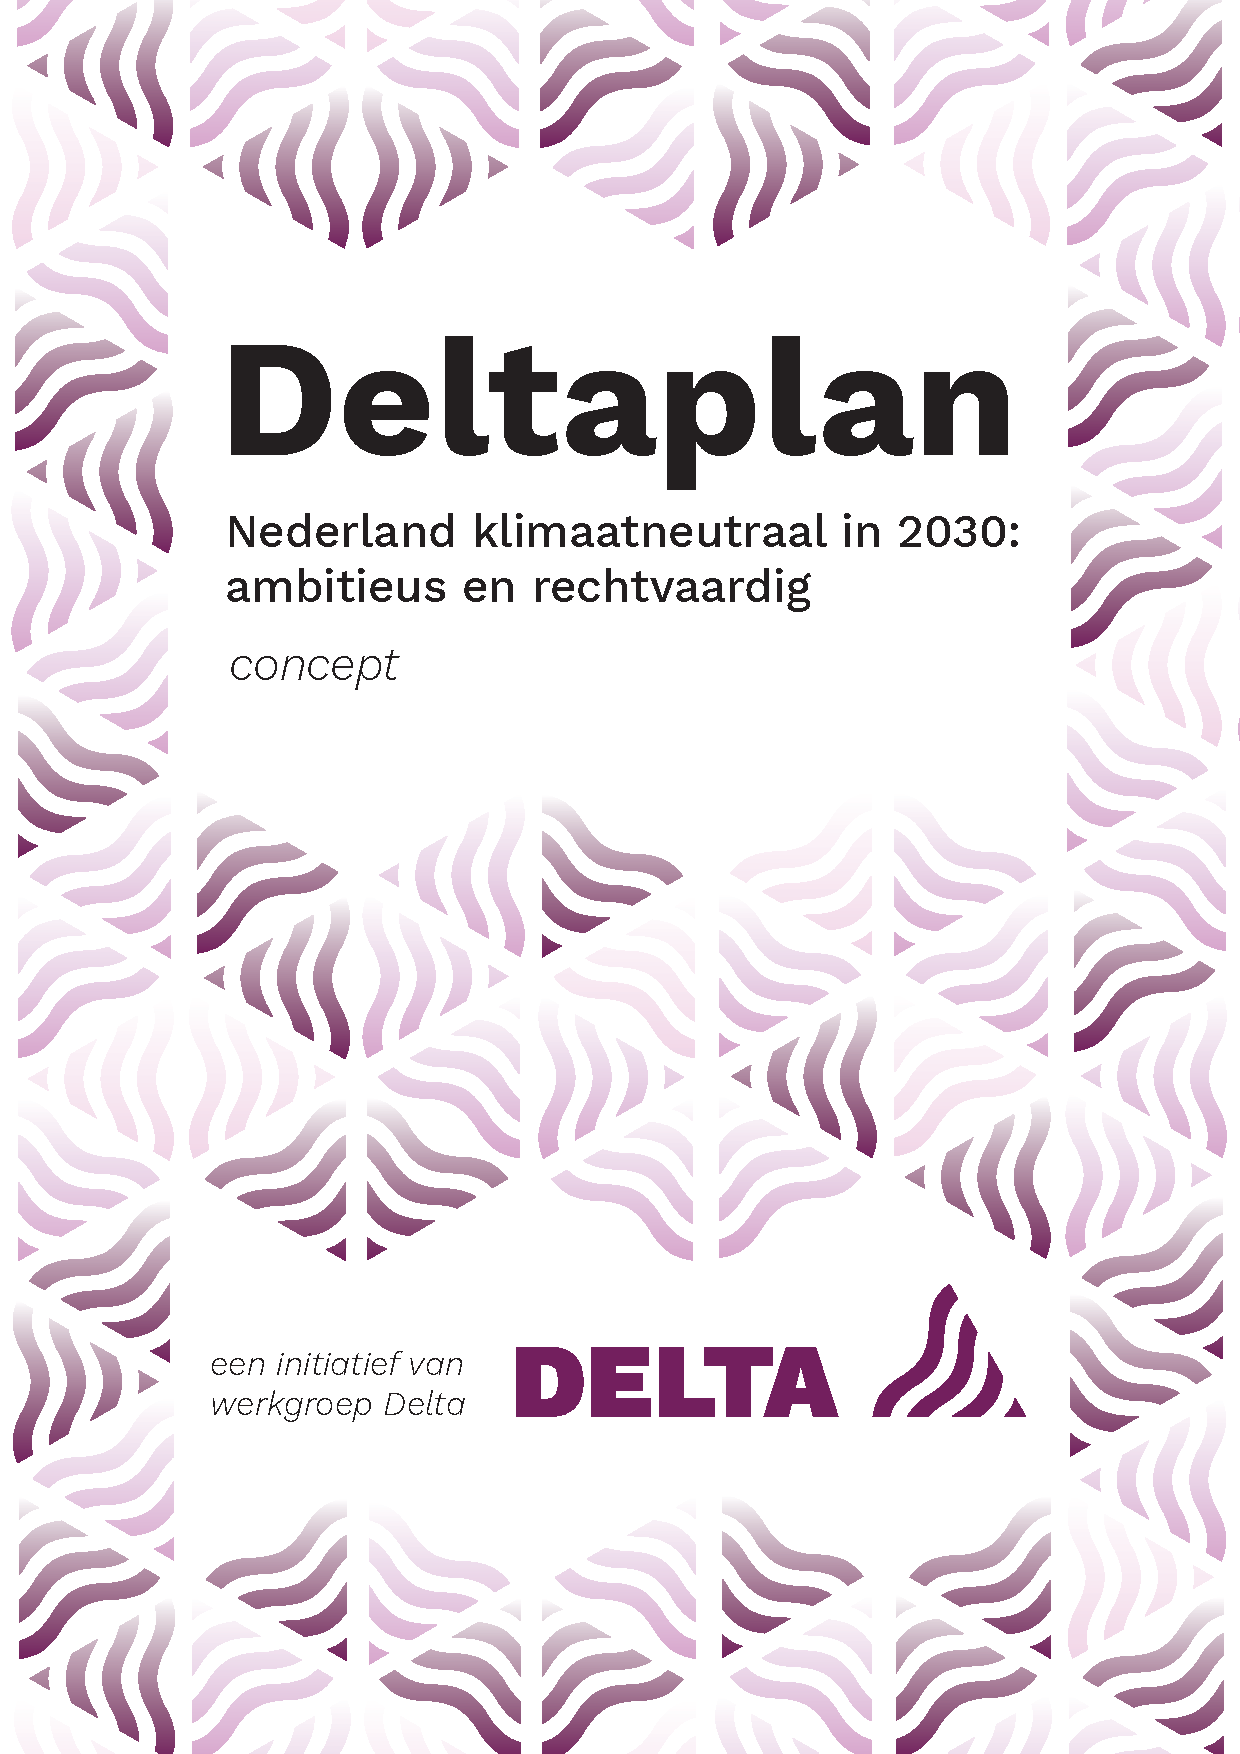
\includepdf[pages=-, pagecommand=\thispagestyle{plain}]{img/frontpage_v5.pdf}

\begin{titlepage}
\makeatletter

\vspace*{15em}

\begin{centering}

	{\Huge \textbf{\@title}}

	\vspace{2em}

	{\Large \textbf{\@subtitle}}

	\vspace{2em}

	{\Large \textit{\concept} (\versionnumber)}

\end{centering}

\vfill

\colofon{Datum}{\@date}
\colofon{Initiatief}{Werkgroep Delta}
\colofon{Eindredactie}{\eindredactie}
\colofon{Bijdragen}{\@author}
\colofon{Contact}{contact@deltagroenlinks.nl}

\makeatother
\end{titlepage}


\tableofcontents

\part{Introductie}
% \chapter{Visieschets}

\chapter{Voorwoord}

\begin{multicols}{2}

Het huidige Nederlandse klimaatbeleid is \emph{te weinig, te laat.}
Daar zullen de meeste groene en linkse mensen het wel over eens zijn.
De klimaatcrisis raakt Nederland op alle vlakken van de maatschappij, maar de respons concentreert zich slechts op relatief smalle ambities en instrumenten.
En die ambities zijn veel te klein: als we de ergste risico's op desastreuze klimaatontwrichting willen voorkomen, moeten we alles op alles zetten om onder de anderhalf graden opwarming te blijven.
Met doelen voor 2050 redden we dat niet: als het aan ons ligt moet Nederland uiterlijk in 2030 volledig klimaatneutraal zijn.

We hebben als Nederland, met onze rijkdom en kennis, een uitgesproken rol te vervullen: in Europa, en in de rest van de wereld.
Dat is niet alleen eerlijk, dat is ook effectief.
Want als we als Nederland weer voorop lopen in de klimaatstrijd, kunnen we andere landen inspireren en meekrijgen.
Door te laten zien dat er alternatieven zijn voor het huidige beleid, creëren we momentum voor een wereldwijde klimaatbeweging.
Daar zit uiteindelijk de meeste slagkracht.

Dat is de oorsprong voor ons Deltaplan: we willen laten zien dat het kán, in 2030 klimaatneutraal zijn.
En dat het ontzettend ingrijpend is, maar we er uiteindelijk een betere, eerlijkere en schonere samenleving voor terug kunnen krijgen.
We richten ons daarbij niet alleen op de technische kant van de transitie, maar benadrukken juist ook het politieke en democratisch verhaal.\footnote{Voor een uitgebreide technische onderbouwing waarom klimaatneutraal in 2030 haalbaar is, wijzen we graag op het uitstekende rapport van Urgenda: \href{https://www.urgenda.nl/visie/rapport-2030/}{\textit{Nederland 100\% duurzame energie in 2030. Het kan als je het wilt}}}
Het is namelijk essentiëel dat de transitie breed gedragen wordt.
Net zoals de Deltawerken ons beschermen tegen het gevaar van het water en we daarmee wereldleider in watertechnologie werden, moeten we ons weren tegen de gevaren van klimaatverandering.
Een nieuwe identiteit voor Nederland staat op het spel.

Dit Deltaplan had niet tot stand kunnen komen zonder de waardevolle bijdrages van onze meeschrijvers.
We zijn hen zeer dankbaar voor het enthousiaste en geïnspireerde meedenken en vormgeven.
Deze conceptversie is een eerste versie van het `levend document' dat het Deltaplan moet zijn: we blijven eraan toevoegen en bijschaven.
Voor nu presenteren we de voorstellen uit het Thema Energie.
Ter inspiratie kun je de gehele lijst met toekomstige voorstellen alvast bekijken in de inhoudsopgave.

We hopen dat dit Deltaplan een begin is voor een nieuwe groene en linkse visie, en we horen graag wat je er van vindt.
Wil je met ons meedenken of meeschrijven? Je kan ons bereiken op \href{mailto:contact@deltagroenlinks.nl}{contact@deltagroenlinks.nl}.

\end{multicols}

\begin{centering}
Met strijdbare groet,\\
\textbf{Jantine, Daan en Rens}\\
\textit{werkgroep Delta}

\end{centering}

% \chapter{Probleemstelling}

% \chapter{Doelstelling}

\chapter{Vertrekpunten}

\begin{mdframed}[
	style=borderless-pink-pastel,
	innertopmargin=15pt,
	innerrightmargin=18pt,
	innerbottommargin=15pt,
	innerleftmargin=18pt
]

{ \setstretch{1.2}
\bfseries \large Het Deltaplan is meer dan een lange lijst voorstellen: het wordt bijeengehouden door een visie voor een rechtvaardige en duurzame samenleving en de weg daarnaartoe. Hieronder leggen we uit vanuit welk standpunt we vertrekken. Het is ons moreel en praktisch kompas in de transitie, en bij alle voorstellen houden we tegen het licht hoe goed ze erin slagen om deze vertrekpunten te realiseren.

}
\end{mdframed}

\begin{multicols}{2}

\vertrekpunt{De overheid zorgt voor de veiligheid van haar burgers}

Een overheid ontleent haar legitimiteit aan het feit dat zij zorg draagt voor het welzijn en de veiligheid van haar burgers. De overheid heeft dus een zorgplicht, en die geldt ook voor het beschermen tegen de gevaren van klimaatverandering. Dit werd recent nog bekrachtigd door de Hoge Raad in de Klimaatzaak die door Urgenda was aangespannen tegen de Nederlandse Staat. De Nederlandse overheid moet dus handelen om klimaatverandering tegen te gaan.

In nauwe relatie tot de zorgplicht staat het voorzorgsprincipe. Dit principe schrijft voorzichtigheid voor bij het handelen in situaties van wetenschappelijke onzekerheid. Wanneer er kans is dat beleid schadelijk is voor de samenleving of het milieu, moet zo worden gehandeld dat dit risico wordt ingeperkt. Dit geldt ook wanneer er nog geen wetenschappelijk waterdicht bewijs is over de aard en de grootte van dit risico. Ook al is er sprake van enige onzekerheid binnen klimaatwetenschappen over de precieze snelheid en onomkeerbaarheid van klimaatverandering, de overheid moet handelen om de potentieel grote risico’s te verkleinen.

\vertrekpunt{Er is geen tijd te verliezen}

We kunnen het ons niet veroorloven om behouden te zijn in de ambitie van de transitie, en we hoeven ook niet te proberen de ‘optimale’ transitiesnelheid te bepalen alvorens te handelen. Die optimale snelheid is namelijk: zo snel mogelijk. Bij gebruikelijke beleidsvraagstukken past het om eerst helder te krijgen wat de verschillende belangen en afwegingen zijn. Maar nu is het zo duidelijk hoe groot de gevolgen traag handelen zijn, dat gecombineerd met het risico op onomkeerbare klimaatdestabilisatie er geen tijd te verliezen is.

Zo hoeven we niet te proberen nu al de energiebehoefte en de beste energietechnologieën voor 2030 te voorspellen: alle duurzame technieken die nu voorhanden zijn, moeten we zo snel mogelijk uitrollen. Beter wedden op te veel dan te weinig paarden. We hoeven niet te wachten tot techniek bewezen en rendabel is voordat we het gaan toepassen. Dat vereist soms een sprong in het diepe en kan soms ook onvoordelig uitpakken als een technologie niet schaalbaar blijkt. Dat is nou eenmaal het gevolg van de noodzakelijke snelheid, en moet ons niet afschrikken.

We zijn behouden over grootschalige toepassingen op korte termijn van technologische ontwikkelingen zoals groene waterstof, biokunststoffen, de Hyperloop, kernfusie, staal gemaakt met waterstof. We proberen ook zonder deze nieuwe technieken een sluitend transitieplan te maken. En tegelijkertijd zijn we groot voorstander van experimenten, innovatie, en het stimuleren van technieken die nog in de steiger staan.

Er is geen maximum doel om te halen, het is geen probleem als we sneller gaan en duurzamer worden dan juridisch strikt noodzakelijk. Immers: als we overschotten aan duurzame energie hebben, of nieuwe, betere technologie waar we niet op gerekend hadden, dan kunnen we daarmee de rest van de wereld vergroenen. Dat is uiteindelijk ook de manier waarop Nederland het meeste impact kan hebben. Als klein land is onze eigen uitstoot in het wereldbeeld gezien beperkt, maar we zijn wel in staat om een sprint te trekken en zo de rest mee te krijgen.

\vertrekpunt{Echte verandering is systeemverandering}

Het is duidelijk dat we niet op de huidige voet door kunnen. De vraag is alleen hoe het anders kan. Het is niet genoeg om individuele burgers aan te spreken hun gedrag. Natuurlijk, uiteindelijk moet iedereen duurzamer eten, kleden, reizen, bouwen. En het is ook goed en belangrijk dat mensen zelf initiatief nemen. Maar het is niet voor individuen weggelegd om het hele systeem te veranderen waarin hun handelen plaatsvindt. We hebben juist politiek nodig om die systeemverandering in te zetten en om te zorgen dat iedereen mee kan bewegen in die transitie.

Politieke actie kan het gehele netwerk raken waarin vraagstukken zich afspelen. Kijk bijvoorbeeld naar een windmolen. Dat is niet alleen een turbine die energie oplevert: het is ook een onderdeel van een internationale grondstoffenketen, die begint bij ijzererts die wordt gemijnd, vervolgens wordt verscheept, wordt gesmolten tot staal dat weer in een andere fabriek wordt gebruikt om de wieken te maken. In elke stap van de keten is er een impact op het milieu, en werken er mensen in zware processen. Ook is een windmolen een object in een landschap: dat kan invloed hebben op de natuur, op de esthetiek, burgers kunnen last hebben van de slagschaduw en het geluid, of zich verbonden voelen met de molen en omarmen als onderdeel van hun omgeving. Iemand is eigenaar van de molen, heeft betaald om hem neer te zetten en er onderhoud aan te laten doen waar weer mensen voor nodig zijn die een goede opleiding moeten hebben gevolgd, en verdient er vervolgens aan.

Elk van die stappen is verbonden met sociale, technische, economische, esthetische, duurzaamheids- en ethische vraagstukken. En in elk van die stappen moet je keuzes maken. Die aspecten negeren zorgt ervoor dat de keuze wordt gemaakt door iemand met andere belangen. Een lokale energiecoöperatie kan wel een windmolen neerzetten, maar kan niet zelf garanderen dat de erts slaafvrij is gemijnd. Het mandaat voor deze keuzes ligt dus bij de politiek.

\vertrekpunt{De overheid is aan zet}

Het initiatief voor de transitie ligt bij de overheid – dat kunnen we niet aan het bedrijfsleven of aan individuele burgers overlaten. Het idee dat sectoren via ‘zelfregulering’ kunnen vergroenen en dat kritische consumenten met hun koopgedrag kunnen aansporen tot duurzame productie, is achterhaald. Het werkt simpelweg niet snel, veelomvattend en transparant genoeg. Daarom geeft de overheid sturing aan de transitie, door doelen te stellen, de weg ernaartoe te schetsen en gepaste instrumenten op stellen zoals subsidies, normen en belastingen.

Daarnaast creëert de overheid ook: ze kan risico’s op zich nemen die niet voor de private sector zijn weggelegd, en zo de wegbereider van een nieuwe markt zijn. Dat doet ze onder andere door het financieren van fundamenteel wetenschappelijk onderzoek, het investeren in nieuwe technologieën en vervolgens de afname van nog niet rendabele implementaties te garanderen, en te voorzien in infrastructuur voor de technologie.

Ten slotte bewaakt de overheid de transitie. Ze controleert of bedrijven zich aan bijvoorbeeld de extra uitstoot- en duurzaamheidsregels houden, om zo een gelijk speelveld te creëren. Daarvoor is het noodzakelijk dat de toezichthouders genoeg middelen krijgen om bedrijven weer echt goed te kunnen controleren.

\vertrekpunt{De transitie creëert gelijkheid}

De noodzakelijke hervormingen van de economie en maatschappij brengen hoge kosten met zich mee en vragen grote offers. Zo zal de consumptie worden ingeperkt, zijn luxeproducten minder vanzelfsprekend en zullen energieprijzen stijgen. Het is essentieel dat de lasten en plichten niet alleen bij de gewone burger terechtkomen. Een klimaattransitie moet dus uit meer dan een lijst van technische oplossingen bestaan. Om de transitie te laten slagen is een massale mobilisatie van motivatie, inzet en talent nodig. Dat kan alleen als iedereen zich in de plannen kan herkennen en zich er een onderdeel van voelt.

Het staat daarom voorop dat de transitie rechtvaardig moet zijn. Dat doet een beroep op solidariteit: de sterkste schouders dragen de zwaarste lasten. Dat is niet alleen eerlijk, het is ook de enige manier waarop de transitie succesvol kan zijn. Nederlanders zouden zich terecht verzetten tegen een transitie die hen onevenredig hard raakt.

Daarom moet de transitie gelijkheid bevorderen. Het is een unieke kans om de economische verhouding weer in balans te brengen. Zo kunnen we energie-armoede tegengaan: door goede isolatie zijn armere huishoudens minder geld kwijt aan de energierekening. We kunnen de belastingen eerlijker en groener maken, en de huizenvoorraad verbeteren. Het maakt de samenleving weerbaarder voor tegenslagen: de komende decennia zullen de gevolgen van klimaatverandering hard beginnen in te slaan. Als mensen bestaanszekerheid hebben, is er meer veerkracht en meer ruimte voor creativiteit. En mensen kunnen makkelijker hun baan verlaten als ze vinden dat deze geen waarde toevoegt om zo werkelijke, duurzame waarde toe te voegen aan de maatschappij.

\vertrekpunt{Burgers zijn eigenaar van de transitie}

De transitie moet meer zijn dan alleen een nationaal opgelegd project. Het is essentieel dat individuele burgers participeren en investeren, en daarvan de vruchten plukken. Dat maakt de verhouding van de winsten gelijk: het wordt zo voor iedereen mogelijk om groen kapitaal op te bouwen. Het voorkomt dat alleen grote investeerders binnenlopen op deze massale economische hervormingen, en dat de ongelijkheid alleen maar toeneemt.

Lokale instrumenten om dit te realiseren zijn bijvoorbeeld gunstige financiering van woningisolatie, het meedoen in een lokale energiecoöperatie, of gezamenlijke deelauto’s in een dorpscollectief. Grotere oplossingen zijn het bouwen van honderdduizenden betaalbare klimaatneutrale woningen, om het voor veel meer mensen mogelijk te maken om vermogen op te bouwen in hun huis. En door bijvoorbeeld alle Nederlanders eigenaar te maken van een gezamenlijk Klimaatfonds waarmee kan worden geïnvesteerd in de transitie. Het zorgt ervoor dat burgers eigenaarschap voelen over het hele plan.

\vertrekpunt{Van product naar recht}

Waar decennia neoliberaal beleid alles van waarde probeert te `verpakken' tot een verhandelbaar product (`commodificatie'), streven wij ernaar de fundamentele onderdelen van ons bestaan weer te zien als een recht. Dat betekent dat iedere Nederlander recht heeft op goed onderwijs, toegang tot zorg, een fijne woning, en openbaar vervoer. De basisbehoeften zoals eten, drinken en kleding moeten voor iedereen betaalbaar zijn. Ook een schone lucht en toegang tot sport- en recreatievoorzieningen en natuur moet vanzelfsprekend zijn. Iedereen moet kunnen beschikken over voldoende vrije tijd en ontspanning. Mensen moeten geen angst hebben voor schulden.

Dat creëert een cultuur en een samenleving waarin immateriële zaken worden gewaardeerd, en onze belangrijkste waarden niet worden uitgedrukt in geld. Er komt meer ruimte voor vrijwilligerswerk en zorg voor elkaar. Het geeft zekerheid en stabiliteit, en daarmee mentale ruimte voor weerbaarheid, creativiteit en welzijn. Het maakt het mogelijk om burgerschap te tonen, om initiatieven te ontplooien en het geeft de tijd om je te mengen in het publieke debat. Zaken die essentieel zijn in tijden van klimaatverandering.

\vertrekpunt{Waardeer publieke investeringen}

De overheid is de belangrijkste investeerder van Nederland. Zo investeert ze in infrastructuur, veiligheid, gezondheid, fundamenteel onderzoek, innovatie, de rechtsstaat, sociale zekerheid en onderwijs. Dat zijn fundamentele drijvers van onze maatschappij. Deze investeringen creëren een stabiele basis voor bedrijven: gezonde en goed geschoolde werknemers, juridische zekerheid, nieuwe technologieën en nieuwe markten waar de overheid de wegbereider van is. De private sector profiteert dus volop van de kracht van de overheid.

Tegelijkertijd geeft het bedrijfsleven te weinig terug aan de samenleving die de investeringen heeft opgebracht. Er wordt op creatieve en soms illegale manier zo weinig mogelijk belasting betaald. Bedrijven zitten vaak op of over de grens van toegestane uitstoot- en milieunormen, en proberen dat te verhullen door groene reclamecampagnes. Met patenten houden ze innovatie die in eerste instantie grotendeels door de overheid is gefinancierd achter voor het publiek. In crisistijd worden grote bedrijven en banken gered, terwijl ze daarna in betere tijden hetzelfde risicovolle gedrag vertonen waar de crisis mee begon. Kortom: de samenleving draagt kosten, maar de winst is voor het bedrijfsleven.

We moeten daarom de overheid weer gaan waarderen als investeerder en schepper van van een goed ondernemersklimaat. Dat betekent dat we erkennen dat de overheid risico mag nemen, en daarin mag falen. En dat de investering van de overheid hoog mogen zijn, omdat de winsten nog hoger zijn en worden verdeeld over de gehele samenleving. Daar staat tegenover dat het bedrijfsleven haar eerlijke deel daarvoor moet betalen met hogere belastingen. En dat ze er niet meer mee weg komt om de regels – over belastingen, concurrentie of milieu – te omzeilen. Dat creëert publieke trots over de kwaliteit en waarde van onze publieke diensten.

\vertrekpunt{Laat groeien wat van waarde is}

Een van de oorzaken van de klimaatcrisis is de manier waarop we succes definiëren en meten. Door een blinde fixatie op het Bruto Binnenlands Product (BBP) als maatstaf voor de economie, en de staat van de economie als maatstaf voor ons algehele succes, zie we niet hoe beperkt zo’n instrument is. Het BBP meet niet hoe duurzaam een land is, hoe gelukkig mensen zijn, hoe zelfstandig burgers zijn. Het BBP stijgt bij elk gasveld dat wordt gevonden en geëxploiteerd, bij elke reparatie door aardbevingsschade, en bij elk vliegtuig dat opstijgt.

We moeten daarom het BBP als instrument en het economisch denken als geheel de deur uitdoen. De staat van de economie is maar een deel van de staat van de wereld. We moeten bepalen wat van waarde is – schone lucht, zelfredzaamheid, een steeds lagere uitstoot, vrij tijd, zorg voor elkaar, vrijheid, natuur, toegankelijke musea, economische gelijkheid – en daar op aansturen. Daarmee verdwijnt de wedstrijd om economische groei, en laten we groeien wat van waarde is.

\vertrekpunt{Betaal de ware prijs}

De prijs van producten en diensten moet de werkelijke prijs reflecteren: niet alleen de kosten die de leverancier heeft gemaakt, maar ook compensatie voor milieu- en sociale schade veroorzaakt door het productieproces. Hiermee verplaats je de kosten van de schade naar de producenten en indirect de gebruiker van het product. Zo krijgt de afnemer een eerlijk beeld van de werkelijke belasting op de aarde en worden duurzame opties aantrekkelijker.

Momenteel zijn veel producten nu goedkoper dan verantwoord is. Denk aan een goedkoop vliegticket, vlees van vee gevoerd met soja waar regenwoud voor is gekapt, en een spijkerbroek waarvan de katoenproductie enorm veel water kost en rivieren vergiftigt. Die schade kan veel vormen aannemen: uitstoot van broeikasgassen, het bedreigen van de leefomgeving van diersoorten, verlies aan biodiversiteit, verontreiniging van water, lucht en bodem, sociale uitbuiting en het aanwakkeren van conflict in instabiele regio's. Doordat deze schade niet is meegerekend in de prijs die ervoor betaald wordt, worden duurzame producten benadeeld.

Er zijn verschillende instrumenten om het speelveld gelijker te maken. Zo kun je producten met een broeikasgasheffing laten betalen voor hun uitstoot met een broeikasgasheffing belasten, of de BTW vervangen door een ‘BTE’: een Belasting Toegevoegde Emissie.  Belangrijk is dat de methode voor zowel bedrijven als consumenten gelijk werkt. Zo is de energiebelasting nu veel hoger voor consumenten dan voor bedrijven, en worden bedrijven niet gedwongen om hun energieverbruik te verlagen. Een ware prijs geldt voor iedereen.

\vertrekpunt{De vervuiler betaalt}

`De vervuiler betaalt' is een drieledig principe: technisch, moreel en praktisch. Technisch of boekhoudkundig betekent het dat belasting van milieuschade of uitstoot wordt betaald door de veroorzaker ervan: een bronbelasting. Moreel zegt het dat vervuilers moeten opdraaien voor de kosten van de vervuiling, en niet de getroffen gebruikers en beheerders van bijvoorbeeld vergiftigde rivieren, dode sloten door overbemesting, of mensen die de gevolgen van klimaatverandering door een hoge CO2-uitstoot ondervinden. De praktische gedachte is dat de grote bedrijven die nu veel uitstoten en de biodiversiteit om zeep helpen, ook de technische en financiële middelen hebben om alternatieven te zoeken en te implementeren. Als je pas later in de keten – bijvoorbeeld bij consumenten in de supermarkt – de verantwoordelijkheid voor duurzame keuzes legt, voelen de verantwoordelijken te weinig noodzaak om hun handelen te veranderen.

\vertrekpunt{Geld dient de werkelijke en duurzame economie}

De afgelopen decennia is geld losgezongen van zijn oorspronkelijke functie: het faciliteren van transacties en de werkelijke economie. Door financialisering – waarbij financiële producten een steeds groter deel van de economische waarde vertegenwoordigen – is de economie losgekomen van de werkelijke waarde en invloed van de onderliggende productieprocessen. Winst en economische groei worden doelen op zichzelf, en geen instrumenten om werkelijke waarde te creëren. De macht van aandeelhouders zorgt voor een kortetermijnvisie, waarbij de focus op kwartaalwinsten het bedrijven onmogelijk maakt om op langere termijn duurzame beslissingen te maken. Daarnaast is de geldscheppende functie van Centrale Banken nauwelijks onderdeel van het politieke debat, terwijl de keuzes daarin niet neutraal zijn.

Het is een politieke vraag hoe je geld inzet en hoe je het financieel systeem ontwerpt. We moeten geld dus zo ‘ontwerpen’ dat het de werkelijke economie dient, en moet zo gereguleerd worden dat het duurzame beslissingen aanmoedigt. Dat is een correctie op de opgeblazen waarde en beloningen voor sectoren zoals flitshandel die geen reële waarde toevoegen, of zelfs waarde vernietigen zoals fossiele bedrijven. De functie van geld verandert daarmee van neutraal gegeven tot onderdeel van het politieke debat.

\vertrekpunt{Niet beslissen óver, maar beslissen met en door}

De transitie kun je niet van hogerhand opleggen. Er zijn talloze vraagstukken die provincies, gemeentes en burgers direct raken. Die hebben impact op bijvoorbeeld onze woningen, de energievoorziening, het landschap en de toegang tot mobiliteit. Het is dus belangrijk om waar mogelijk beslissingen lokaal te maken. Uitbreiding van lokale verantwoordelijkheid moet altijd gepaard gaan met uitbreiding van lokale macht en middelen – het mag nooit een verkapte bezuinigingsoperatie zijn.

Zo laat je ook ruimte over voor lokaal initiatief. Het is essentieel dat wooncorporaties, burgerinitiatieven en energiecoöperaties ruim baan krijgen om de transitie zelf vorm te geven. Dat vergroot niet alleen de waardering voor de veranderingen, het maakt het ook nog beter en sneller om er nieuwe oplossingen komen en iedereen meewerkt. De ambities en middelen moeten centraal worden vastgesteld, de implementatie zoveel mogelijk decentraal.

\vertrekpunt{Internationale rechtvaardigheid is leidend}

Klimaatverandering en verlies van biodiversiteit leiden tot natuurrampen, voedseltekorten, droogtes en conflicten. De landen die het hardst worden getroffen door deze klimaatcrisis hebben vaak het minst bijgedragen aan het ontstaan ervan. De veroorzakers hebben daarentegen meestal minder last van de nadelige effecten van klimaatveranderingen, door een gunstiger geografische ligging en meer middelen voor klimaatadaptatie. Nederland behoort met haar historisch gezien hoge uitstoot bij de veroorzakers van de klimaatcrisis. We hebben dus een verantwoordelijkheid om internationaal rechtvaardig klimaatbeleid aan te jagen. Dat berust op drie pijlers: ten eerste schroeven we zo snel mogelijk onze huidige uitstoot terug en sporen we andere rijke landen aan om hetzelfde te doen. Vervolgens ondersteunen we anderen landen in klimaatadaptatie, om zo de gevolgen van onder andere droogtes en natuurrampen tegen te gaan. Ten slotte compenseren we voor geleden en toekomstige schade als gevolg van klimaatverandering. Hiermee toont Nederland haar solidariteit in de internationale klimaatstrijd.


\end{multicols}


\part{Voorstellen}
\part{Voorstellen}

\thema{Energie}

\begin{visie-concept}{Visie op energie}\end{visie-concept}

\begin{voorstel}{Flexibiliteit van het net}
\meeschrijver{Otto Barten}

\begin{samenvatting}
Om klimaatneutraal te worden, moeten we de flexibiliteit van het net zo goed mogelijk benutten. Op dit moment komt dit onvoldoende uit de verf, vooral omdat de overheid de prikkels niet goed heeft gezet. Delta bepleit meer flexibele contracten en een overheid die gaat beprijzen op basis van \COO-uitstoot. Burger en bedrijfsleven worden zo gestimuleerd om zelf de flexibiliteit te ontwikkelen die ons klaarmaakt voor 100\% klimaatneutraal!
\end{samenvatting}

\begin{multicols*}{2}
\raggedcolumns

\begin{uitdaging}
In de klassieke stroommarkt volgt de opwek van elektriciteit de vraag: fossiele centrales worden op- en af geregeld om genoeg stroom te leveren. Als onze opwek grotendeels van windmolens en zonnepanelen komt, fluctueert het aanbod echter, en kan dit aanbod de vraag maar beperkt volgen. We moeten dus proberen om zoveel mogelijk onze elektriciteit te gebruiken wanneer de duurzame opwek het grootst is: als het waait en de zon schijnt. Dat is ook belangrijk om de piekbelasting van het net te verkleinen. Hoe zorgen we ervoor dat de vraag het aanbod gaat volgen?
\end{uitdaging}

\begin{overwegingen}
% Deze flexibilisering gebeurt nu al in pilots\footnote{https://vandebron.nl/elektrisch-rijden/slim-laden}\footnote{https://www.tennet.eu/nl/nieuws/nieuws/tennet-na-succesvolle-pilots-door-met-blockchain/}\footnote{https://www.elaad.nl/projects/slim-laden-in-de-praktijk/}\footnote{https://www.deltares.nl/nl/nieuws/project-slim-malen-komt-op-stoom/} en op kleine schaal\footnote{https://www.jedlix.com/nl/}\footnote{https://www.laadje.nl/ (dit product is ontwikkeld door het bedrijf van de auteur)}, maar dit moet de standaard worden. De overheid kan hier met name voor zorgen door de prikkels in het systeem goed te zetten. Op dit moment zijn de prikkels voor het flexibel gebruiken van elektriciteit namelijk vaak nog te gering, waardoor minder \COO uitstoten of de netten ontlasten niet altijd beloond wordt.

\paragraph{Flexible energiecontracten}
Op dit moment is de elektriciteitsvraag grotendeels inflexibel. Hoewel de prijs van elektriciteit voor energieleveranciers zelf al varieert, hebben veel huishoudens een contract met één vaste prijs of hooguit dag- en nachttarief. Dat betekent dat ze geen prikkel hebben om stroom te verbruiken wanneer er duurzame opwek is, en ruimte op het net. Er is een EU-richtlijn die voorschrijft dat elke energieleverancier de optie moet aanbieden aan consumenten om variabele prijzen te betalen \parencite{europees_parlement_notitle_nodate}. Deze prijzen zijn lager als er veel duurzame opwek is. Zo kan de burger er voor kiezen om deel te nemen aan dit slimme elektriciteitsnet. Deze richtlijn wordt nu echter niet door Nederland gehandhaafd.

\begin{infobox}{Wat is een slim elektriciteitsnet?}
Een slim elektriciteitsnet of \term{smart grid} is een netwerk met apparaten die zichzelf automatisch aanzetten wanneer er veel duurzame opwek, en ruimte op het net is. Zo houdt het net zichzelf in balans en gebruiken we zo veel mogelijk duurzame energie.
\end{infobox}

\paragraph{Huishoudens}
Huishoudens kunnen zelf het tijdstip van hun elektriciteitsvraag aanpassen, door bijvoorbeeld op een ander tijdstip de wasmachine of de vaatwasser aanzetten. Nog grotere impact maakt het om de elektrische auto op een ander tijdstip op te laden of de warmtepomp even uit te zetten als er een piek in de vraag optreedt of als er weinig duurzaam vermogen is. Elektrische auto’s kunnen zelfs gaan terugleveren op deze tijden. Burgers moeten zelf kunnen kiezen welke slimme oplossingen ze kiezen. Misschien besluiten straks de meeste mensen dat ze best hun elektrische auto ‘s nachts op kunnen laden als ze daar een vergoeding van 1 euro per keer voor krijgen, maar dat ‘s nachts de was doen voor 5 cent per keer te onhandig is. Dat is uiteraard prima.

\paragraph{Bedrijfsleven}
Het bedrijfsleven nam in 2017 69\% van het elektrisch verbruik voor z’n rekening \parencite{centraal_bureau_voor_de_statistiek_statline_nodate}. Dat aandeel zal waarschijnlijk groeien door elektrificatie van industriële processen. Hier zit ook het grootste deel van de flexibiliteit. Voorbeelden van industriële apparaten die te verschuiven zijn in de tijd zijn: koelings- en verwarmingsapparaten, e-boilers, gemalen, kassen en warmte-krachtkoppelingsinstallaties (WKK). Ook een bedrijf kan zelf besluiten of het verbruik verschoven wordt: misschien kan dit wel bij een koelbedrijf of een tuinder, maar niet bij een telecomaanbieder.

\paragraph{Prijsprikkels}
De flexibiliteit van het net berust op een marktprincipe: de vraag reageert op de prijs. Het is dan essentiëel dat de prijs ook eerlijk is en duurzame energie aantrekkelijk maakt.

Op dit moment is dat maar gedeeltelijk zo.

Het is niet aan de overheid om deze beslissingen direct te nemen, maar wel om bedrijven aan te sporen. Dit moet de overheid in de eerste plaats doen met het invoeren van afdoende prikkels zoals \COO-heffingen, zodat er voldoende vraagsturing plaatsvindt. Naast de \COO-heffing kan de overheid er ook voor kiezen om de energiebelasting niet op basis van kWh te heffen, maar op basis van \COO. Ook dit zorgt voor veel extra flexibiliteit.

Deze flexibiliteit kan ervoor zorgen dat we in de zomer ‘s avonds en ‘s nachts het surplus van zonne-energie benutten dat overdag wordt opgewekt. Ook een dag met wat minder zon moeten we, met bijvoorbeeld de batterijen van onze elektrische auto’s, kunnen overbruggen zonder dat er centrales aangezet hoeven te worden. In de winter kunnen we één of twee windstille dagen overbruggen. Alleen als de wind in de winter langer niet thuis geeft, hebben we zo onze aardgas-, biomassa- of waterstofcentrales nog nodig.

\paragraph{Grotere pieken} Een tweede uitdaging is dat een groeiend deel van ons energiegebruik in de vorm van elektriciteit is, om industrie processen worden geëlektrificeerd, en we steeds meer elektrische auto’s en warmtepompen hebben. De belasting van ons net wordt daarmee groter. Zo zorgen alleen al de 2,8 miljoen elektrische auto’s, die met het huidige beleid in 2030 verwacht worden, dat de piekvraag met bijna 50\% groeit, als de flexibiliteit van het stroomnet niet benut zou worden \parencite{enpuls_slim_2019}.


\begin{infobox}{Seizoensflexibiliteit}
Flexibilisering van de netten kan wonderen doen op de korte termijn, van minuten tot enkele dagen. Maar op seizoensschaal kan flexibilisering weinig bijdragen. Ook opslag in bijvoorbeeld waterstof of accu’s is hiervoor duur. Wat handiger is, is om de hoeveelheid zonnepanelen, die vooral ‘s zomers produceren, en windparken, die vooral ‘s winters stroom leveren, slim op elkaar af te stemmen. Zo hebben we waarschijnlijk maar weinig opslag nodig!
\end{infobox}

\begin{infobox}{Lokale congestie}
Als de prikkels op nationaal niveau goed gezet worden, worden hiermee gelijk ook de pieken in de lokale netten verminderd. Op lokaal niveau kunnen er soms wel andere bottlenecks zijn, bijvoorbeeld als de hele straat zijn auto oplaadt wanneer er veel windenergie wordt opgewekt. Als deze pieken apart verminderd moeten worden, kunnen regionale netbeheerders gebruikmaken van bestaande regionale markten, zoals GOPACS, waarop slimme apparaten kunnen worden aangesloten. Ook kan bekeken worden of slimme contracten, waarbij de aansluitkosten gelijke tred houden met het maximaal gevraagde vermogen, een oplossing zijn.
\end{infobox}

\paragraph{De prijs van stroom}
Als de overheid [deze punten] uitvoert, ontstaat een situatie waarbij stroom fors duurder wordt op momenten waarop er onvoldoende duurzame energie wordt opgewekt. Maar gemiddeld hoeven we niet meer te gaan betalen: de stroomprijzen dalen juist sterk als er voldoende wind en zon is. Hierdoor wordt zowel de burger als het bedrijfsleven in gelijke mate gestimuleerd om te verbruiken op tijden waarop er zoveel mogelijk duurzaam aanbod is, en zo weinig mogelijk vraag. Dit houdt de benodigde netinvesteringen relatief laag en reduceert de behoefte aan piekvermogen in de vorm van vervuilende aardgascentrales, impopulaire biomassacentrales of dure groene waterstof. Zo werkt het flexibele net optimaal mee en wordt het bereiken van 100\% duurzaam zo eenvoudig en goedkoop mogelijk!


\end{overwegingen}

\begin{aanbevelingen}
\speerpunt{Verplicht stroomaanbieders om al hun klanten de optie te geven voor flexibele tarieven.} om variabele prijzen te gaan betalen, en zo deel te gaan nemen aan het smart grid.

Stimuleer dat zowel consumenten als bedrijven hier gebruik van maken, en dat ze een zo groot mogelijk deel van hun verbruik flexibel maken.

- open standaarden

\speerpunt{Zorg dat de energieprijs is gebaseerd op de \COO-uitstoot van de opwekking, en dat deze voor iedereen gelijk is.}

- CO2 belasting (bij vervuiler!)

- energiebelasting op basis van CO2

- ETS

Beloon flexibel energiegebruik door de energiebelasting te heffen op \COO-basis, niet op kWh-basis. Er kan veel flexibiliteit gegenereerd worden door de belasting op deze basis te heffen bij de energiecentrale in plaats van bij de verbruiker.

Zet daar bovenop zwaar in op het EU-ETS: zorg dat ook deze \COO-beprijzing veel hoger en universeel wordt (geen gratis rechten meer). Ook dit is cruciaal om de flexibiliteit te ontsluiten die nodig is voor 100\% duurzaam

Om koolstoflekkage te voorkomen naar werelddelen met een minder ambitieuze klimaatpolitiek, moet op Europees niveau een importheffing (en eventueel exportsubsidie) op \COO-basis ingevoerd worden. De interne broeikasbelasting kan dan zo hoog worden als nodig, zonder dat er banen verdwijnen naar landen met een minder ambitieuze klimaatpolitiek. 

Benut deze hervormingen om zowel groot- als kleinverbruik hetzelfde bedrag per uitgestoten ton \COO te laten betalen. Gelijke monniken, gelijke kappen. Dit zorgt voor een rechtvaardige energietransitie die aan mensen uit te leggen valt. Zorg dat de burger zich niet hoeft af te vragen waarom de energietransitie haar veel geld kost, maar de raffinaderij van Shell buiten schot blijft.

\speerpunt{Stimuleer ontwikkeling van flexibele oplossingen.}

\speerpunt{Garandeer de privacy voor burgers.}
\end{aanbevelingen}

\end{multicols*}

\end{voorstel}

\begin{voorstel}{Wind op Zee}
\meeschrijver{Rens Baardman}

\headerimg[Prinses Amaliawindpark voor de kust van IJmuiden][\copyright{} Ad Meskens \CC{} BY-SA]{img/energie/wind-op-zee-header}
% https://commons.wikimedia.org/wiki/File:Prinses_Amalia_windmolenpark_4.jpg

\begin{samenvatting}
Verdriedubbeling van ambitie zorgt voor schone energie die een toevoeging is voor de Noordzee-natuur. Burgers profiteren daar ook financiëel van.
\end{samenvatting}

\begin{multicols}{2}

\begin{uitdaging}
Momenteel brengen de windmolens op de Noordzee 1 GW aan elektriciteit op. Met de huidige plannen wordt dit ruim 11 GW in 2030, 12\% van het huidige elektriciteitsverbruik. Een mooi aandeel, maar er is nog veel meer potentie. Zeker als de vraag naar stroom toeneemt door elektrificatie van de industrie en auto’s, is wind op zee cruciaal om op een duurzame manier aan die vraag te voldoen. Hoe kunnen we meer elektriciteit opwekken uit windenergie op zee? Hoe zorgen we dat de natuur en individuele burgers kunnen profiteren van de parken?
\end{uitdaging}

\begin{overwegingen}
\paragraph{Windparken}
Een windpark op zee bestaat uit tientallen tot honderden windmolens met een capaciteit van 5 à 10 MW per stuk. De windmolens zijn via lange kabels op de bodem van de zee verbonden met het hoogspanningsnet aan de wal. De opgewekte stroom kan met grote omvormers op zee worden omgezet van wissel- naar gelijkstroom voordat het naar land wordt getransporteerd. Er zijn voorstellen om kunstmatige eilanden te bouwen waar de omvormers kunnen staan, bijvoorbeeld bij de Doggersbank, een ondiepte ver in de Noordzee. Hier leggen dan netbeheerders uit Duitsland, Denemarken en Nederland samen een internationaal knooppunt voor windenergie en waterstof aan \parencite{north_sea_wind_power_hub_north_2019}. Zo’n `energie-eiland' zou ook dicht bij de Nederlandse kust kunnen worden gebouwd. Net als de Marker Wadden is zo’n eiland een kennis- en excursiecentrum met bezoekers en een bijzondere plek voor natuur en biodiversiteit.

\begin{infobox}{Wat betekent \term{capaciteit}?}
De capaciteit van een windmolen duidt op het maximaal op te wekken hoeveelheid stroom als er veel wind staat. De behaalde opbrengst is afhankelijk van de daadwerkelijke windsterkte. Gemiddeld over een jaar behaalt een windmolen zo’n 50\% van de maximale capaciteit \parencite{lensink_kosten_2017}. Dat levert op jaarbasis bijna 44 GWh op, genoeg elektriciteit voor 16.000 huishoudens.
\end{infobox}

\paragraph{Planning en aanleg}
Vanaf het eerste initiatief kan het tot wel tien jaar duren voordat een windpark is aangelegd \parencite{westra_offshore_2014}, en kost honderden miljoenen euro’s. Het proces begint met de tenderfase waarbij de overheid kavels selecteert waar geïnteresseerde bedrijven een voorstel voor kunnen doen. Daarna volgt ontwerp, aanleg en aansluiting. Vanaf dan kan het park zeker 20 jaar rendabel draaien \parencite{lensink_kosten_2017}. Sinds 2018 zijn alle tenders subsidieloos. Alleen de netaansluiting naar het land is voor de rekening van de netbeheerder, en daarmee voor de staat.

\paragraph{Locaties op de Noordzee}
Nieuwe windparken kunnen worden gebouwd binnen de Exclusieve Economische Zone: een gebied dat anderhalf keer zo groot is als Nederland, dat Nederland mag exploiteren. Windparken worden niet aangelegd in de gebieden die nodig zijn voor scheepvaartroutes, zandwinning, visserij, militaire terreinen en natuurgebieden. Ook moet de zee niet te diep zijn: vaak wordt 30 meter als maximum gehanteerd. Daarnaast wil je de parken het liefst dicht bij de kust hebben staan, zodat de elektriciteitsverbinding naar de wal niet te duur wordt, en niet te dicht bij de kust, zodat je de parken niet ziet. Alsnog zijn er nog veel geschikte gebieden over. Het Planbureau voor de Leefomgeving schetste al een scenario waarbij in 2050 voor 60 GW aan Nederlandse windmolens is geïnstalleerd \parencite{matthijsen_toekomst_2018}.

\paragraph{Natuur}
De aanleg van windparken is een kans voor natuur op de Noordzee. Tussen windmolens wordt niet gevist, waardoor de zeebodem, riffen en daarmee biodiversiteit kunnen herstellen.  De fundering van windmolens zijn ook goede aanhechtingsplaatsen voor oesters en ander bodemleven. Er lopen experimenten om in windparken kunstriffen te maken \parencite{didderen_offshore_2019}. Ook opent zich een weg naar ‘zeeboerderijen’ (aquacultuur): tussen de windmolens kunnen krabben, kreeften, oesters, mosselen en zeewier worden gekweekt.
Belangrijk is dat (bruin)vissen, zeehonden, vogels en vleermuizen zo min mogelijk last hebben van de molens. Dat kan met geluiddempende bellenschermen om windmolens heen tijdens de aanleg, nieuwe hei-technologie die minder lawaai maakt, en het preventief uitzetten van turbines als er vogels of vleermuizen worden gedetecteerd.

\paragraph{Burgerparticipatie}
De Noordzee en de wind die daar waait zijn ons collectief natuurlijk kapitaal, dus niet alleen grote ontwikkelaar, maar juist alle burgers hebben recht op het dividend daarvan. Burgers, energiecoöperaties, pensioenfondsen en lokale overheden moeten dus mee profiteren. Burgerparticipatie is een belangrijk onderdeel van het Klimaatakkoord, maar is nog geen criterium bij de tenderprocedures. Bij wind op land is burgerparticipatie al veel gebruikelijker \parencite{nwea_gedragscode_2016}.

\end{overwegingen}

\begin{aanbevelingen}

\speerpunt{In 2030 staat er op de Noordzee voor 30 GW aan windmolens.}
Dat is een verdriedubbeling van de huidige ambitie in het Klimaatakkoord. Die versnelling wordt gerealiseerd door het rap uitgeven van grote, nieuwe kavels. Door het stimuleren van technische ontwikkelingen stijgt de capaciteit per windmolen. Een stevige \COO-belasting maakt windprojecten nog aantrekkelijker voor ontwikkelaars, zodat kavels straks geveild kunnen worden. Die opbrengsten gaan in een nationaal Klimaatfonds en worden gebruikt om nieuwe parken te financieren.

\speerpunt{Burgerparticipatie wordt een voorwaarde} in de tenderprocedure, zodat burgers bij kunnen dragen aan minstens 20\% van de investeringen voor een park.
Dat kan bijvoorbeeld via het Klimaatfonds of met lokale energiecoöperaties. Zo worden alle Nederlanders mede-eigenaar van onze stroomvoorziening.

\speerpunt{Windmolenparken worden een aanwinst voor de Noordzee-natuur.}
Onderzoek naar herstel van zeebodem en -leven wordt gestimuleerd. Zeeboerderijen zijn een alternatief voor de huidige visserij.

\speerpunt{Kunstmatige energie-eilanden} zijn nieuwe natuurgebieden, met faciliteiten voor recreatie, een haven voor pleziervaart, en kenniscentra van waaruit (school)excursies worden georganiseerd.
We laten zien waar onze energie vandaan komt, maken duidelijk hoe de transitie er fysiek uitziet, en het creëert trots op onze duurzame infrastructuur.

\end{aanbevelingen}
\end{multicols}

\end{voorstel}
\begin{voorstel}{Wind op land}
\meeschrijver{Bram van den Groenendaal}

\headerimg[Windmolenpark in Soest vanuit de lucht][\copyright{} L-BBE \CC{} BY]{img/energie/wind-op-land-header}
% https://commons.wikimedia.org/wiki/File:Soest,_Netherlands_-_panoramio_(12).jpg

\begin{samenvatting}
De groei van windenergie op land is cruciaal voor de energietransitie. We verdrievoudigen daarom het opgestelde vermogen tot 2030. Draagvlak en inpassing in het landschap zijn cruciaal. Een investering in energie moet daarom een investering zijn in toekomstperspectief voor de regio.
\end{samenvatting}

\begin{multicols}{2}

\begin{uitdaging}
Windenergie op land is onmisbaar in de energietransitie. In 2019 stond er voor ruim 3,5 GW aan vermogen, zo’n 2000 windmolens \parencite{cbs_statline_nodate}. Dat is nog ver onder de doelstelling van 6 GW in 2020 uit het Energieakkoord van 2013 \parencite{rijksoverheid_windenergie_2016}. Windparken op land zijn nu vaak later klaar dan gepland. We moeten de capaciteit dus sterk opschroeven. Hoe zorgen we ervoor dat dat gaat lukken? En hoe passen we dat in in het landschap, en met medewerking van burgers?
\end{uitdaging}

\begin{overwegingen}
\paragraph{Windmolens op land}
Wanneer we het hebben over wind op land gaat het over zowel kleine windmolens die enkele huishoudens van elektriciteit voorzien, als de meer gangbare windturbines van zo'n 3 MW. De innovatie en efficiëntie in de windsector maakt echter dat turbines steeds groter, hoger en efficiënter worden en dus meer opwekken. Daarom wordt er tegenwoordig gerekend met grote windturbines van 5 tot 6 MW per stuk. De keuze voor het type turbine is afhankelijk van de lokale omstandigheden (ruimte, netbelasting, draagvlak, etc.). Wanneer meerdere (vaak grote) windturbines bij elkaar staan spreken we van een windpark.

\paragraph{Planning en locaties}
Op dit moment worden op tientallen plekken in Nederland windmolen(parken) ontwikkeld, vaak op plekken die zijn aangewezen als kansrijke gebieden door overheden of worden aangedragen door lokale initiatiefnemers. Tot 2030 wordt er gewerkt aan Regionale Energiestrategieën; in 30 regio’s worden plannen gemaakt voor de opwekking van wind- en zonne-energie. Hierin worden gebieden aangewezen die kansrijk zijn voor windenergie. De aanleg van windparken op land is gecompliceerd en duurt daarom lang. Een initiatiefnemer gaat door verschillende fases: een verkennings-, vergunnings- en realisatiefase. Die kunnen bij elkaar wel negen jaar duren \parencite{rijksdienst_voor_ondernemend_nederland_windenergie_nodate}.

Of een locatie kansrijk is hangt af van verschillende zaken. Allereerst van de andere al aanwezige functies. Zo is men over het algemeen terughoudend met het ontwikkelen in natuurgebieden of bij archeologische vindplaatsen en zijn er beperkingen in de buurt van bebouwing, vanwege het geluid, de slagschaduw en het fysieke risico. Daarnaast wordt er gekeken naar de afstand tot en de capaciteit van het elektriciteitsnet om te garanderen dat het project technisch en financieel haalbaar is. Ook wordt er gelet op de inpassing en het landschap, en de opstelling van de windmolens. Zo kunnen locaties langs snelwegen of bedrijventerreinen of in bepaalde typen landschappen de voorkeur hebben boven andere locaties.

\paragraph{Het initiatief}
Anders dan bij windmolens op zee, ligt het initiatief voor een windmolenproject [meestal] niet bij de overheid. TODO

\paragraph{Kosten en financiering}
De ontwikkeling van een windpark kost niet alleen tijd, maar vraagt ook om vele onderzoeken, ruimtelijke procedures, overleg met omwonenden en andere belanghebbenden. Dan zijn er nog de bouwkosten van het windpark, de aanschaf van de windturbines, de netinpassing en de kosten van beheer en onderhoud als het windpark eenmaal draait. Er zijn zodoende subsidies beschikbaar (SDE+) om windmolenparken te ontwikkelen. Er wordt echter ook aan windmolens verdiend. Zo krijgen grondeigenaren vaak een vergoeding voor het gebruik van hun grond en verdienen de initiatiefnemers aan de exploitatie. Een stelregel is dat grootschalige opwek kostenefficiënter is dan kleinschalige opwek.


\paragraph{Draagvlak en participatie}
Het draagvlak staat bij windenergie vaak onder druk; mensen voelen zich niet gehoord of vinden dat initiatieven van bovenaf worden opgelegd. Zonder draagvlak worden processen langzaam of stranden ze. Participatie in zowel het proces, als in de exploitatie is daarom een cruciale voorwaarde. Dit kan op vele manieren. Zowel via inspraak in de reguliere politieke processen als door directe participatie in het maken van de plannen. Ook financiële participatie is een bewezen middel om het draagvlak te versterken. Zo kunnen bewoners investeren in het park door aandelen te kopen of door via een energiecoöperatie (mee) te ontwikkelen. Er zijn nu al meer dan 500 coöperaties actief met 35.000 à 40.000 leden en het aantal is groeiende (RVO, 2020). Tegelijkertijd bestaat het risico dat een aanpak met vele kleinschalige initiatieven een ‘confetti’ aan windmolenparken oplevert \parencite{college_van_rijksadviseurs_via_2019}. We moeten zodoende op zoek naar een aanpak die werkt voor het draagvlak en het landschap.
\end{overwegingen}

\begin{aanbevelingen}
\speerpunt{We verdrievoudigen het huidige vermogen van windenergie op land.}
Om tot 2030 de weg te bereiden naar een energieneutrale samenleving moet de opwek van windenergie op land fors groeien. Volgens de scenario’s van het PBL en Urgenda moeten we uitgaan van zeker een verdrievoudiging van het huidige vermogen, naar zo’n 11 GW. We willen de verdrievoudiging realiseren door de bouw van windmolenparken met de modernste windmolens (op dit moment gaan we uit van zo’n 5,6 MW) en het herstructureren van bestaande parken met verouderde molens.

\speerpunt{We clusteren wind op land op passende locaties.}
Om zo het landschap zo veel als mogelijk te sparen en daarmee het draagvlak voor duurzame energie te vergroten. We ontkomen er niet aan ook in het open landschap windparken te ontwikkelen, bij voorkeur op locaties waar het veel en hard waait en in grootschalige polderlandschappen. Zo voorkomen we een hagelslag aan kleine windparken en behouden we de (economische)schaalvoordelen van clustering. Draagvlak voor een dergelijke ontwikkeling is essentieel.

\speerpunt{We brengen de baten en lasten van windenergie bij elkaar.}
Tegenover een grote bijdrage aan verduurzaming van een regio moet een vorm van (financiële) compensatie staan. Afspraken over grootschalige opwek werken zo twee kanten op. We trekken hierbij lessen uit de Europese Green Deal, waar er via een ‘Just Transition Mechanism’ extra investeringen gaan naar regio’s die harder worden geraakt door de transformatie naar een groene economie. Ook moeten partijen uit de regio zoals burgers, ondernemingen en overheden verplicht kunnen deelnemen in de investeringen, en dus ook het rendement.

\speerpunt{We zoeken de verbinding met andere opgaven in de regio.}
Verduurzaming van regio’s zou niet alleen moeten bijdragen aan het verminderen van de \COO-uitstoot, maar bijdragen aan versterken van een toekomstperspectief. Juist in de landelijke regio’s van Nederland waar veel ruimte is voor duurzame opwek spelen andere uitdagingen, zoals bevolkingskrimp of economische stagnatie. Investeren we alleen in wind en zon, maar niet in de mensen, dan roept dat weerstand op. Denk aan de exploitatie van gas in Groningen of de grote windparken in Drenthe. Mensen moeten voelen dat investeringen in verduurzaming naast een verandering van het landschap ook bijdragen aan een betere toekomst. Als verduurzaming ook een investering is in betere mobiliteit of meer regionale banen komt dat het draagvlak ten goede.

\speerpunt{Overheden doen het vooronderzoek, zodat kleinere partijen makkelijker mee kunnen doen.}
[Geinspireerd op de tenders voor Wind op Zee. Hoe juridisch haalbaar is dit? TODO]
\end{aanbevelingen}

\end{multicols}


\end{voorstel}

% \begin{voorstel}{Zonnepanelen op daken}
\meeschrijver{Krik van Zwet}

\begin{samenvatting}
Zonnepanelen moeten op alle bedrijfsgebouwen geïnstalleerd worden
\end{samenvatting}

\begin{multicols*}{2}

\begin{uitdaging}
Het streven is er op gericht om zonnepanelen te plaatsen op zo veel mogelijk daken van bedrijfsgebouwen. Bedrijfsgebouwen zijn meestal groter dan particuliere woonhuizen en bieden daarom plaats aan grote aantallen zonnepanelen.
\end{uitdaging}

\begin{overwegingen}
Er gebeurt al heel veel op het terrein van zonnepanelen. Naast particulieren, energiecoöperaties (postcode-roos-projecten) en overheden zijn er zeker ook bedrijven, die duurzaamheid als leidraad gebruiken om energie op te wekken middels zonnepanelen. Zonnepanelen op daken ontsieren het landschap minder, indien de zonnepanelen worden geplaatst op hoge gebouwen. Hoge gebouwen zijn in de regel bedrijfsgebouwen, zoals b.v. distributiebedrijven. Plaatsing van zonnepanelen op dit soort hoge gebouwen heeft dus twee voordelen, t.w.

\begin{enumerate}
	\item de aantallen zonnepanelen zijn groot
	\item de zonnepanelen zijn aan het oog onttrokken.
\end{enumerate}

Probleem hierbij is, dat veel bedrijven en investeerders, die dit soort gebouwen in eigendom hebben of laten bouwen, vanuit zichzelf niet overtuigd zijn van nut en noodzaak van de plaatsing van zonnepanelen.
\end{overwegingen}

\begin{aanbevelingen}
Er moet daarom een wet komen, die bedrijven verplicht om op de alle daken van hun bedrijfsgebouwen (oudbouw en nieuwbouw) vóór 1 januari 2025 zonnepanelen te installeren. Deze wet is nodig, omdat het overtuigen van de bedrijven van de noodzaak om groene energie op te wekken te lang gaat duren en ook nog eens bij te veel bedrijven niet zal lukken. Er is geen tijd meer voor eindeloos overleg.
\end{aanbevelingen}

\end{multicols*}

\end{voorstel}

\begin{voorstel}{Zonnepanelen op velden}
\meeschrijver{Edo van Baars}

\headerimg[Zonnepark Lange Runde in de buurt van Emmen][\copyright{} 44BART44 \CC{} BY-SA]{img/energie/zonnepanelen-op-velden-header}
% https://commons.wikimedia.org/wiki/File:ZLRLaag.jpg
% TODO: "Tegen de bouw van dit zonnepark en meerdere parken in met name het noorden van Nederland wordt bezwaar gemaakt door bewoners die vrezen voor grootschalige aantasting van het landschap." (https://nl.wikipedia.org/wiki/Zonnepark_Lange_Runde)

\begin{samenvatting}
Zonneparken worden zorgvuldig in het landschap ingepast. Zonneparken worden een plek waar biodiversiteit op de voorgrond staat. Ontwikkelaars investeren in natuur, biodiversiteit en educatie. De regio stelt eisen aan de ontwikkeling en de burger besluit mee over de investeringen van ontwikkelaars.
\end{samenvatting}

\begin{multicols}{2}

\begin{uitdaging}
In het Nationaal Klimaatakkoord is afgesproken dat in 2030 35 TW aan elektriciteit op land worden opgewekt door wind op land en zonnepanelen op velden en grote daken [i]. Grootschalige projecten waarin zonnepanelen op velden worden gebouwd, ook wel zonneparken genoemd, zijn nu al commercieel al erg aantrekkelijk [ii]. Ook in de Regionale Energie Strategieën spelen zonneparken een belangrijke rol.

Naar verwachting zal de energieproductie van zonnepanelen toenemen van 1,5 TW in 2018 naar 8,5 TW in 2030. Niet alle daken zullen geschikt zijn voor zonnepanelen en de ruimte in bebouwd gebied is al schaars. Overigens worden zonneparken meer rendabel, naarmate ze groter worden in omvang. [iii] Het is daarom aannemelijk dat zeker een kwart van de zonnepanelen dus op veld zal komen te liggen. [iv]

Hoe plaatsen we in de toekomst zonnevelden in het landschap met respect voor de natuur en in samenspraak met de lokale bevolking?
\end{uitdaging}

\begin{overwegingen}
\paragraph{De Zonneladder}
We kunnen er niet omheen dat de klassieke zonneparken impact hebben op de natuurlijke omgeving. Een zonnepark heeft een industriële uitstraling, die niet goed past tussen natuur en groene landbouwgrond. De Zonneladder is een nieuw toetsingsinstrument dat een richtlijn geeft over waar zonnepanelen te plaatsen. Zonnepanelen worden met voorkeur op de daken en gevels geplaatst of in bebouwd gebied, zoals bij parkeerplaatsen en geluidsschermen langs de weg. Daarna pas komt de plaatsing in natuur-en landbouwgebieden. De voorkeur ligt dan bij locaties zoals waterzuiveringsinstallaties, vuilnisbelten, of bermen van wegen. [v]
\paragraph{Natuur rondom het zonnepark}
Door grootschalige ruilverkaveling medio 20e eeuw zijn kleine kavels opgebroken en natuurlijke afscheidingen – zoals houtwallen – weggehaald. Juist houtwallen bieden beschutting voor vogels, egels, vossen en insecten. Door houtwallen rondom zonnevelden verplicht te maken, gaan zonneparken bijdragen aan biodiversiteit.  Op het zonnepark komen nauwelijks mensen en vervoersmiddelen waardoor dieren vrij spel hebben.

\paragraph{Groen rondom het zonnepark}
Verschillende groene elementen van het landschap kunnen in en rondom het zonnepark worden geïncorporeerd. Dijken, watergangen, houtwallen, paden of bomenrijen zorgen ervoor dat het park meer in de omgeving opgaat. Het strakke patroon van het park wordt doorbroken. Verzekeraars vragen dat zonneparken kunnen worden afgesloten. In plaats van een hek, kan een groene heg,  houtwal of brede watergangen worden gebruikt. Een groene afscheiding zorgt voor minder zichtbaarheid van het park en geeft het landschap meer diepte, het biedt een spannender en afwisselender aanzicht dan een leeg, ruim verkaveld landschap.

\paragraph{Biodiversiteit in het park}
De bodem onder zonnepanelen kan verschalen, doordat water en zonlicht niet bij de grond kunnen.  Maar er zijn ook manieren waarop zonneparken een kans kunnen zijn voor natuur en biodiversiteit.  Door voldoende ruimte tussen de panelen te laten kan de biodiversiteit worden versterkt, bijvoorbeeld wanneer er mossen kunnen groeien, die goed met schaduw kunnen omgaan. Regenwater kan ondanks de panelen alsnog de bodem bereiken. Zo droogt de grond niet uit en krijgt het bodemleven weer een kans. [vi]

Bij nog meer ruimte tussen de panelen kunnen er schapen en kippen worden gehouden. Insectenhotels, bijenkorven en nestkasten kunnen tussen de panelen worden geplaatst. Het graven van kleine poelen tussen en naast panelen kan ook andere flora en fauna trekken. De functie van een zonnepark kan zelfs nog breder worden getrokken. Door wandelpaden door de zonnevelden aan te leggen, wordt het een plek om te recreëren. Schoolklassen kunnen zonnevelden bezoeken om te leren over al het bodemleven en duurzame energie.[vii]

\paragraph{TODO: geld voor de natuur}
[Om de 5\%-regeling te onderbouwen]

\end{overwegingen}

\begin{aanbevelingen}
We gaan ontwikkelaars van zonneparken verplicht om 5\% van de investering naar verbetering van het landschap te laten gaan. Dit wordt opgenomen in de Zonneladder. Het is geïnspireerd op de Percentageregeling voor Beeldende Kunst (1\% investeringsvereiste in beeldende kunst bij nieuwbouw/verbouw van overheidsgebouwen). De gemeente en de provincie kunnen deze aanvullende eis stellen aan de ontwikkelaar als het bestemmingsplan moet worden gewijzigd.  Zo kan er lokaal worden gekeken welke eisen precies nodig zijn.  Bewoners krijgen een stem in de besteding van de 5\%.  Dit geld kan worden geïnvesteerd in natuurlijke afscherming, educatie of versterking van biodiversiteit.  Het  risico op landschapsschade wordt omgezet in verbetering van het landschap.
\end{aanbevelingen}


\paragraph{Literatuur}
[i] Rijksoverheid (2019). Nationaal Klimaatakkoord – elektriciteit. Link: \url{https://www.klimaatakkoord.nl/elektriciteit}

[ii] Ploum Rotterdam Law Firm (2019). De zonneladder komt eraan: Realisatie nieuwe zonneparken aan banden gelegd . Link: https://www.ploum.nl/de-zonneladder-komt-eraan-realisatie-nieuwe-zonneparken-aan-banden-gelegd/)

[iii] Spruijt, J. (2015). Wat levert een Zonneweide per ha op? Link: https://edepot.wur.nl/336567

[iv] Nationaal Programma RES (2019). Factsheet Zon-pv en wind op land Analyse naar opwek van hernieuwbare energie per RES-regio. Link: https://www.regionale-energiestrategie.nl/documenten/handlerdownloadfiles.ashx?idnv=1460717

[v] Tweede Kamer (2018). Motie van het lid Dik-Faber c.s. over een zonneladder opstellen in samenspraak met decentrale overheden. Link: \url{https://www.tweedekamer.nl/kamerstukken/moties/detail?id=2018Z17050&did=2018D46309}

[vi] Zee, van der et al. (2019). Zonneparken – natuur en landbouw. WUR. Link: https://edepot.wur.nl/475349

[vii] BAR-Organisatie (2019). Concept - Ruimtelijke verkenning Zonneparken in het buitengebied.

\end{multicols}

\end{voorstel}



\begin{voorstel}{Waterstof}
\meeschrijver{Mark Leenen}

\headerimg{img/energie/waterstof-header}
% https://commons.wikimedia.org/wiki/File:Berkhof_Ambassador_op_waterstof.jpg
% TODO: zijn we wel fan van waterstofbussen?

\begin{samenvatting}
In 2030 wordt groene waterstof gebruikt als energiebron als aanvulling op duurzamere en efficiëntere energiebronnen, zoals zon- en windenergie. Door de ontwikkeling van een waterstofeconomie worden veel banen gecreëerd. Wereldwijd is Nederland koploper in waterstoftechnologie.
\end{samenvatting}

\begin{multicols*}{2}

\begin{uitdaging}
Waterstof is een gas dat gebruikt kan worden als opslagmiddel voor energie (elektriciteit), of als brandstof voor industriële processen op hoge temperatuur, of als grondstof voor de (chemische) industrie. Via brandstofcellen kan waterstof omgezet worden in elektriciteit, bijvoorbeeld voor de aandrijving van elektromotoren in de transportsector. 
Er wordt onderscheid gemaakt tussen grijze, blauwe en groene waterstof. Waterstof wordt momenteel vooral gemaakt uit koolwaterstoffen zoals aardgas. Dit wordt grijze waterstof genoemd, omdat er  CO2 vrijkomt. Wanneer de vrijgekomen CO2 wordt opgeslagen, wordt gesproken van blauwe waterstof. Door met elektriciteit watermoleculen te splitsen, kan waterstof ook worden geproduceerd zonder CO2 uitstoot. Dit is groene waterstof. Idealiter is de elektriciteit die wordt gebruikt duurzaam opgewekt. Vaak worden groene waterstof en windmolenparken op zee in 1 adem genoemd.

Nederland is momenteel na Duitsland al de grootste producent van waterstof in Europa, met een productie van 8 miljard m3 per jaar. Deze (grijze) waterstof is vooral bedoeld als grondstof voor de chemische industrie, en zal de transitie moeten maken via blauw, naar groen. Alle infrastructuur die geschikt is voor grijze of blauwe waterstof, is ook geschikt voor groene waterstof.

Groene waterstof is alleen rendabel bij voldoende schaalgrootte. Die schaalgrootte kan alleen ontstaan bij voldoende vraag. Vraag en aanbod moeten samen gestimuleerd worden om de waterstofeconomie van de grond te krijgen.

Waterstofgas heeft andere eigenschappen dan aardgas (methaan). Technische uitdagingen zitten in het geschikt maken van delen van het aardgasleidingnetwerk voor waterstof. En in de toepassing van waterstof als brandstof in hoog-temperatuur processen in de industrie.
\end{uitdaging}

\begin{overwegingen}

Waterstof is een energie-opslag medium. Het opslaan en vrijmaken van energie in waterstof kost ook energie. Qua energie-efficientie scoort waterstof geen hoge ogen en zal daarom alleen een rol spelen in decarbonisatie van processen en sectoren waar decarbonisatie op andere manieren (zoals directe elektrificering) niet mogelijk is. Gedurende de jaargetijden waarin zonnepanelen veel energie opwekken, en in tijden van veel wind(energie), kan het overschot opgeslagen worden in de vorm van waterstof. In de maanden waarin weinig zonne-energie opgewekt wordt, of wanneer het minder waait, wordt het tekort dan aangevuld vanuit waterstof.

Nederland is goed gepositioneerd om een leider te worden in de waterstofeconomie. De Noordzee biedt gelegenheid voor grote windparken, waarvan de duurzame elektriciteit gebruikt kan worden voor elektrolyse van water tot groene waterstof. Nederland heeft een bestaande gas-infrastructuur die deels geschikt gemaakt kan worden voor waterstof. En Nederland heeft een sterke logistieke en chemische sector, waar waterstof goed in zal passen. Daarnaast heeft Nederland grote lege gasvelden, waar CO2 in opgeslagen kan worden vanuit de productie van blauwe waterstof.

Windparken op zee zullen een belangrijke rol spelen in de waterstofproductie. Op zee kunnen electrolyzers worden aangedreven met de opgewekte elketriciteit om waterstof te maken. In het verlengde daarvan kan transport van waterstofgas, boven transport van electriciteit, een kostprijsvoordeel opleveren [hy-gro].

Waterstof kan een belangrijke rol gaan spelen in internationaal vrachtverkeer. Deze sector heeft zich verenigd in de European Clean Trucking Alliance (ECTA). Al vanaf 2021 kan de Total Cost of Ownership van een vrachtwagen die rijdt op waterstof, concurreren met diesel. Vanaf 2021 kan ook langzaam accijns geheven worden op waterstof, om de investeringen in de waterstofeconomie terug te gaan verdienen. Vrachtwagens die waterstof verbruiken kunnen mede door Nederlandse bedrijven ontwikkeld en gebouwd worden (DAF en Scania, Holthausen Clean Technology). Ook in de scheepvaart wordt de toepassing van waterstof onderzocht, zoals in het Blue Dolphin project. [Hydrogen4climateaction.eu]

De lancering van de European Clean Hydrogen Alliance (ECH2A) op 8 juli 2020 laat zien dat Europa vol op waterstof in wil zetten. In Hydrogen Europe is de complete productieketen voor waterstof vertegenwoordigd door 160+ bedrijven, inclusief Nederlandse spelers. Ook lopen er al projecten om groene waterstof van en naar Nederland te transporteren (Green Spider, Green Flamingo \& H2Go, hydrogen4climateaction.eu).

In de industrie zal waterstof een rol spelen als brandstof voor industriële processen die een temperatuur > 250 C nodig hebben [Quintel]. Die processen zijn namelijk moeilijk direct te electrificeren. Momenteel wordt waterstof al bijgemengd bij methaan voor zulke processen. Ook kan waterstof op termijn biomassa vervangen als brandstof. Waterstof kan ook in plaats van methaan als grondstof dienen voor productie van kunstmest, en toepassing in de staalindustrie biedt eveneens mogelijkheden tot decarbonisatie.

Het huidige gasnet wordt aangepast en uitgebreid, zodat het in 2030 ook deels gebruikt kan worden voor transport van waterstof. Die waterstof is echter vrijwel niet bestemd voor huishoudens, maar grotendeels voor de industrie en het transport. In de gebouwde omgeving is een zo klein mogelijke rol voorzien voor waterstof. Hier blijft “gasvrij” het credo, tenzij dat niet kan en een CV ketel op waterstof de beste oplossing blijkt (zoals voor oudere woningen die niet op een warmtepomp over kunnen vanwege slechte isolatie). Waterstof moet zoveel mogelijk worden getransporteerd via pijpleidingen en niet via trucks. Voor afstanden < 1000 km is de efficiëntie van transport van waterstof door pijpleidingen zeer goed (>95\%). [BOSSEL]

\end{overwegingen}

\begin{aanbevelingen}
De windparken op zee moeten in de toekomst een mix van elektriciteit en groene waterstof (middels electrolysers op zee) leveren.
Er moet een landelijk waterstof pijpleiding netwerk gerealiseerd worden waarop alle grote afnemers (industrie, transport) aangesloten worden. Het bestaande gasnet dient hiervoor als basis.

Zwaar transport (vrachtvervoer) stapt over op waterstof als brandstof, met toegewijde waterstoftankstations langs snelwegen, die aangesloten zijn aan het waterstof gasnet. Voor inclusie van internationaal transport is het onontbeerlijk om de waterstofeconomie op Europees niveau te ontwikkelen. Particulier, lokaal en streekvervoer maakt in beginsel geen gebruik van waterstof als energiedrager, maar rijdt op batterijen.

Waterstof wordt gebruikt als brandstof in hoog-temperatuur processen in de industrie. Eerst zal blauwe waterstof worden gebruikt als geschikte tussenoplossing. Blauwe waterstof wordt lokaal geproduceerd en opgeslagen. Wanneer mogelijk wordt de overstap naar groene waterstof gemaakt. In de loop van de komende decade kan groene waterstof al bijgemengd worden bij blauwe of grijze waterstof, om vraag voor groene waterstof te creëren.

\end{aanbevelingen}

\paragraph{Literatuur}
http://hydrogeneurope.eu

http://hy-gro.net

Wind-to-hydrogen (W2H2) TKI Systeemintegratie Studie TES1216101

https://www.flightglobal.com/air-transport/forget-batteries-is-hydrogen-the-holy-grail-for-carbon-free-commercial-aviation/139150.article

\url{https://www.nrc.nl/nieuws/2020/07/08/brussel-omarmt-waterstof-a4005372#/handelsblad/2020/07/09/#301}

Ulf Bossel, “Does a hydrogen economy make sense?”, Proceedings of the IEEE, Vol. 94, No. 10, 2006, 1826 - 1837

J. Reijerkerk and G. van Rhee, “Waterstof: kansen voor de Nederlandse industrie”, Oktober 2019

https://clean-trucking.eu/publications/europes-opportunity-to-decarbonise-the-road-freight-sector/

http://www.hydrogen4climateaction.eu

Commissie Economische Zaken en Klimaat, “Kabinetsvisie Waterstof en Routekaart Groen Gas: Position Papers Reader”, 7 mei 2020

Institute for Sustainable Process Technology, “Hychain 1,2 \& 3: Energy carriers and hydrogen supply chain”, december 2019

https://www.portofrotterdam.com/nl/havenkrant/havenkrant-43/grootste-groene-waterstoffabriek-van-europa

https://www.natuurenmilieu.nl/themas/energie/projecten-energie/waterstof/waterstof-de-waterstofladder/

\end{multicols*}

\end{voorstel}

% \begin{voorstel}{Biomassa}
\meeschrijver{Renaat van Rompaey}

\begin{samenvatting}
Tegen 2030 gebruiken we alleen nog biomassa en hout dat duurzaam geproduceerd is én hergroeit.  Het gebruik ervan wordt schoon en veilig.  Ook in Nederland zorgt Groenlinks tegen 2030 voor twee keer zoveel bos en bomen.
\end{samenvatting}

\begin{uitdaging}
Momenteel leidt het gebruik van biomassa vaak tot natuurvernietiging en niet-duurzaam bosbeheer (Cardellichio et al. 2010). Het is belangrijk dat we het gebruik weten te beperken tot de hoeveelheid die duurzaam geproduceerd kan worden. In Nederland kunnen we twee maal zoveel hout en biomassa produceren als we op dit moment doen en tegelijk genieten van de vele bijkomende voordelen zoals waterberging, zuivere lucht, klimaatkoeling, schaduw en habitat voor biodiversiteit.

Vuur en rook zijn ook bronnen van luchtvervuiling, brengen gevaar met zich mee en kunnen schadelijk zijn voor de gezondheid, hoewel de mens er al een miljoen jaar mee omgaat. Samen rond een houtvuur brengt mensen opnieuw in contact met elkaar, vlammen zijn mooi om naar te kijken, directe warmte is behaaglijk, het creëert gezelligheid.
\end{uitdaging}

\begin{overwegingen}
\paragraph{Vuur}
Sinds meer dan één miljoen jaar heeft de mens geleerd het vuur te beheersen en gebruiken. Als brandstof gebruikte hij gedroogde plantenresten en hout. Nog tot op de dag van vandaag is gedroogde biomassa de belangrijkste brandstof voor het grootste deel van de wereldbevolking en het duurzaam gebruik ervan één van de grootste uitdagingen van de groene transitie.

\paragraph{Hout}
Hoewel biomassa kan slaan op om het even welk weefsel van natuurlijke oorsprong (mest, slib, voedselresten, dierlijke vetten, slachtafval, landbouwafval, zagerijafval; Kamerstuk 35 167, 22-11-2019,), beslaat hout het merendeel van de biomassa die we hier bedoelen. Hout geeft stevigheid aan planten en laat ze toe honderd meter hoog te groeien en duizenden jaren oud te worden. Voor het stenen tijdperk was er al een ‘houten tijdperk’, toen de mens leerde van hout en vezels allerlei gebruiksvoorwerpen (wapens) en behuizing te maken. Hout is onze belangrijkste grondstof en is, na olie, het belangrijkste wereldhandelsproduct (wto.org).

\paragraph{Duurzaam beheerd bos}
Het meeste hout groeit in bossen. Groenlinks is voor duurzaam bosbeheer. Niet alleen groeit er in duurzaam beheerde bossen evenveel hout bij als er gekapt wordt, maar daarnaast vervult het bos er ook haar andere functies, zoals habitat/thuis voor biodiversiteit, bodemvormer, waterberger in de watercyclus, luchtzuiveraar, klimaatkoeler, bron van voedsel en medicijnen, biotoop (leuke plek om te zijn) voor de mens (en zijn huisdier). Het bos in al zijn verschijningsvormen en gradaties is onmisbaar voor de mens. Erbuiten ligt alleen de steppe, de woestijn, het hooggebergte, de toendra en de poolstreken, waar het te droog, te heet, te zout of te koud is voor bomen om te groeien.

Groenlinks is voor bosbehoud. De mens heeft al te veel ontbost, voor landbouw, mijnbouw, infrastructuur, steden en bebouwde oppervlakte, wegen, industrie. Daarnaast heeft de mens bijna alle bosecosystemen op de wereld overbenut, overgebrand, en overgeëxploiteerd. Groenlinks wil dat de ontbossing stopt en dat bosherstel plaatsvindt. Bossen kunnen herplant worden, beschermd worden, duurzaam beheerd worden. In Nederland en buitenland is Groenlinks voor natuurherstel, natuurbouw soms, en natuurbescherming, door natuureducatie, multifunctioneel landgebruik en respect voor het leven op aarde en de natuurlijke processen die onze landschappen vormgeven tot ware kunstwerken van de natuur. De levende wezens zijn afhankelijk van elkaar voor hun voortbestaan en leven in symbiose op deze aardbol.

\paragraph{Biomassa als product van duurzaam bosbeheer}
Hout is een prachtig natuurproduct en wordt al te vaak vervangen door metaal, plastic of beton. We moeten zuinig zijn op hout en bosproducten die duurzaam geproduceerd zijn. Hergebruik en recyclage verdienen de voorkeur boven verbranding.

Om onze hele energievoorziening op biomassa te laten lopen, zijn enorme oppervlakten bos nodig. De ruimte is echter schaars op plekken waar voldoende regen valt opdat er bos zou groeien. Op diezelfde plekken willen we aan landbouw en veeteelt doen voor onze voedselvoorziening. Bij gebrek aan ruimte in Nederland, halen we het uit het buitenland.

In het buitenland gelden andere, soms minder strenge wetten en zo zien we dat er in het buitenland veel natuur verdwijnt of bos niet-duurzaam beheerd wordt om aan de Nederlandse vraag te voldoen. Groenlinks is voor eerlijke wereldhandel, met respect voor de natuur. Importeurs  moeten dit aantonen zodat de stromen niet-duurzaam geproduceerde producten verkleinen, wat dan weer de prijs kan verhogen.

\paragraph{Duurzaam, maar ook te duur om op te stoken}
En zo komen we tot de slotsom: duurzaam geproduceerde biomassa is duur en zal dus geen mirakeloplossing zijn om Nederland klimaatneutraal te maken. Er zijn andere goede redenen om in Nederland meer bomen te krijgen en meer bos te hebben. Groenlinks is voor natuurlijke bosverjonging met inheemse soorten. Dat levert robuustere en gevarieerde ecosystemen op, beter bestand tegen wind, vuur, water, vraat en zelfs het nieuwe klimaat. Tien procent bosbedekking in Nederland is echt te weinig. Wij willen twintig procent bosbedekking in 2030.

Bij verzagen van boomstammen naar planken houd je maar dertig procent van het oorspronkelijke volume over. De houtverwerkende industrie heeft dus een hoop afvalhout en - zaagsel en dat moet zo nuttig mogelijk hergebruikt worden. Verbranding voor terugwinning van de opgeslagen energie zou de laatste optie moeten zijn.

\paragraph{Biomassa in de energietransitie: alleen goede biomassa, als het niet anders kan, en zonder subsidie}
Voor zover biomassa in de energietransitie gebruikt moet worden, moet het goede biomassa zijn, ongesubsidieerd, en voor hoogwaardige toepassingen of piekvermogen. Er moet dus gecontroleerd worden of de biomassa niet leidt tot ontbossing, verslechterde bodem- of waterkwaliteit, verlies van biodiversiteit, verminderen van voedsel- en waterzekerheid, of schendingen van mensenrechten. Daarnaast moet er een duidelijk positief klimaateffect zijn, bijvoorbeeld bij piekvermogen minstens 70\% minder CO2-uitstoot dan aardgas binnen een bosherstelperiode van tien jaar. Biomassa die niet aan deze criteria voldoet, mag niet in Nederland gebruikt worden. Biomassa die wel aan deze criteria voldoet, mag gebruikt worden, maar alleen voor hoogwaardige toepassingen of piekvermogen. Stroomopwek met biomassa is dus alleen een optie als er niets anders beschikbaar is, bijvoorbeeld in enkele windstille winterweken per jaar. Warmteketels leveren basislast en deze mogen dus niet meer op biomassa draaien.\footnote{Zie ook https://www.natuurenmilieu.nl/wp-content/uploads/2020/07/Biomassa-Visie-2020.pdf}

\paragraph{Schoon stoken}
Het stoken van hout in de open haard brengt veel fijnstof in de lucht. De Gemeente Den Haag heeft \href{https://www.denhaag.nl/nl/in-de-stad/natuur-en-milieu/duurzaamheid/verstandig-hout-stoken.htm}{9 tips om zo schoon mogelijk te stoken.} Zo gaan de tips onder andere over het aanschaffen van de juiste kachel, aanmaakmethode en een schone schoorsteen. Bij ongunstige weersomstandigheden, zoals weinig wind en mist, blijft rook langer hangen. Met een stookalert roept het RIVM mensen op om dan geen hout te stoken.

\paragraph{Veilig barbecueën}
Bij verbranding en verkoling van biomassa voor de barbecue komen verschillende kankerverwekkende stoffen (zoals heterocyclische amines en polycyclische koolwaterstoffen) vrij je beter niet opeet of aan je vingers krijgt. De \href{https://www.kanker.be/alles-over-kanker/aantoonbaar-risico/tips-om-gezonder-te-barbecue-n}{Stichting tegen kanker heeft tips voor een gezonde barbecue.} Groenlinks promoot zelfredzaamheid. \href{https://www.kanker.be/alles-over-kanker/aantoonbaar-risico/tips-om-gezonder-te-barbecue-n}{Kamperen is de mooiste zomersport,} waardoor je steeds maar jonger wordt. Weten hoe je in de natuur (over)leeft, hoort ook bij een ecologische levenswijze, dus wonen, zich verwarmen, koken (ook water koken) in de natuur, hoort daarbij.

\end{overwegingen}

\begin{aanbevelingen}
\speerpunt{Tegen 2030 gaan we duurzaam met biomassa om. De bossen waaruit we biomassa winnen, worden duurzaam beheerd.}
Er komt op de wereld veel biomassa vrij bij ontginningen en landgebruikconversie, maar ook bij laan- of fruitbomen die vervangen worden. Als daarvoor de correcte vergunningen afgegeven zijn, hoeft dat hout niet ‘fout’ te zijn en is zorgvuldig gebruik ervan, geen probleem. Maar elk lucratief gebruik kan leiden tot overexploitatie, dus de overheid moet zijn rol als regulator vervullen.

\speerpunt{Elektriciteitsproductie met biomassa kan alleen bij garantie dat het duurzaam geproduceerd is én hergroeit.}
Voor hout en dus ook pellets geldt dat  het legaal geproduceerd moet zijn (EU Timber Regulation) om ingevoerd te kunnen worden in de EU. Nu is legaliteit nog geen garantie voor duurzaamheid, maar het verwijst wel dat er rekening gehouden is met de rurale bevolking of inheemse volkeren en dat de natuurbeschermingswetten niet geschonden zijn.

Jong, hergroeiend bos legt veel CO2 vast en als de Nederlandse subsidie verstrekt wordt onder veronderstelling van CO2-vastlegging van alle uitstoot van die centrales, dan moet dat ook zijn gecertificeerd. 

\speerpunt{Elektriciteitsproductie met biomassa wordt alleen gebruikt wanneer er langdurig geen andere duurzame energie voorhanden is.}
Dat kan bijvoorbeeld in een windstille winterweek zijn.

\speerpunt{We gebruiken alleen goede biomassa.}
Dat betekent dat alleen biomassa die niet leidt tot ontbossing, verslechterde bodem- of waterkwaliteit, verlies van biodiversiteit, verminderen van voedsel- en waterzekerheid, of schendingen van mensenrechten, gebruikt mag worden. Ook moet de biomassa binnen tien jaar bosaangroeitijd minstens 70\% klimaatvriendelijker zijn dan aardgas.

\speerpunt{Biomassa heeft geen subsidie meer nodig.}
De huidige subsidies worden uitgefaseerd. De nieuwe, goede biomassa hoeft niet gesubsidieerd te worden, omdat deze alleen wordt ingezet voor hoogwaardige toepassingen of piekproductie van elektriciteit, die mede dankzij de gestegen CO2-belasting toch al hoge opbrengsten geeft.

\speerpunt{Biomassa gebruiken we niet voor warmteopwek.}
Opwek van stadswarmte is laagwaardig gebruik, en biomassa is hier te schaars voor. Subsidies voor warmteopwek met biomassa worden dan ook stopgezet en nieuwe warmteprojecten mogen geen biomassa meer voor basislast warmteopwek gebruiken.

\speerpunt{Aanzienlijke herbebossing en bosherstel tegen 2030 houden Nederland leefbaar bij klimaatverandering en herstelt onze waterbalans, zuivert onze lucht, verkoelt en verrijkt de biodiversiteit.}
Nederland is veel te kaal. Langs wegen, waterlopen en langs perceelsgrenzen kan veel bos, struweel en houtkanten verschijnen. Groenlinks wil een boomrijke leefomgeving met twee keer zoveel bomen in 2030 binnen en buiten de bebouwde kom. De bebouwde kom moet ontstenen en ontharden. Na de bloemrijke wegbermen verschijnt er ook een bloem- en boomrijke binnenstad met groendaken. Subsidies voor monocultuur-landbouw moeten omgebogen worden naar landschapszorg en kleinschalige voedselproducerende gemengde systemen.

\end{aanbevelingen}

\paragraph{Literatuur}
Cardellichio, P.; et al. (2010). Walker, T. (ed.). "Massachusetts Biomass Sustainability and Carbon Policy Study: Report to the Commonwealth of Massachusetts Department of Energy Resources" (PDF). Natural Capital Initiative Report NCI-2010-03. Brunswick, Maine.: Manomet Center for Conservation Sciences.

Kamerstuk 35 167, 22-11-2019, Regels voor het produceren van elektriciteit met behulp van kolen (Wet verbod op kolen bij elektriciteitsproductie),

V. Cram Martos \& F. Romig. Trade in energy and forestry, a perspective from the United Nations Economic Commission for Europe. Contribution from the United Nations Economic Commission for Europe

https://www.natuurenmilieu.nl/wp-content/uploads/2020/07/Biomassa-Visie-2020.pdf

De Dagelijkse Standaard, 20 mei 2020. Jesse Klaver claimt dat GL tegen biomassa is, wordt voor paal gezet met allerlei pro-biomassa GL-wethouders. https://www.dagelijksestandaard.nl/2020/05/jesse-klaver-claimt-dat-gl-tegen-biomassa-is-wordt-live-voor-paal-gezet-met-allerlei-pro-biomassa-gl-wethouders/

Minister Wiebes, 17-10-2019. Memorie van antwoord wetsvoorstel Wet verbod op kolen bij elektriciteitsproductie. https://www.rijksoverheid.nl/documenten/rapporten/2019/10/17/regels-voor-het-produceren-van-elektriciteit-met-behulp-van-kolen-wet-verbod-op-kolen-bij-elektriciteitsproductie

35 167. Regels voor het produceren van elektriciteit met behulp van kolen (Wet verbod op kolen bij elektriciteitsproductie)

\url{https://nl.wikipedia.org/wiki/Menselijke_vuurbeheersing}

\end{voorstel}

\begin{voorstel}{De rol van de RES}
\meeschrijver{Walter Wittkamp}

\headerimg[][\copyright{} Mike Moore \CC{} 0]{img/energie/rol-van-de-res-header}
% https://commons.wikimedia.org/wiki/File:FEMA_-_32463_-_SBA_at_Findlay_Town_Meeting_in_Ohio.jpg
% TODO: get a picture of a real citizens assembly!

\begin{samenvatting}
In de Regionale Energiestrategieën moet burgerparticipatie voorop staan om de burger eigenaar van de transitie te maken. Burgerberaden zullen een belangrijke rol spelen om tot adequaat, haalbaar en rechtvaardig klimaatbeleid te komen.
\end{samenvatting}

\begin{multicols*}{2}

\begin{uitdaging}
In het klimaatakkoord zijn dertig energieregio’s opgericht waar provincies, gemeenten en waterschappen een plan maken over de vergroening van de energievoorziening van hun regio. In deze Regionale Energiestrategieën (RES) ligt de nadruk op duurzame elektriciteit uit zon en wind, verwarming van gebouwen, en alle infrastructuur die daarvoor nodig is. De conceptvoorstellen zijn eind 2020 door elke regio ingediend, nu moet de gemeente aan de slag.
Participatie van inwoners heeft in dit proces echter nog nauwelijks plaatsgevonden. En de tot nu toe gepresenteerde plannen zijn niet ambitieus en dwingend genoeg om de klimaatcrisis aan te pakken.
Hoe zorgen we ervoor dat burgers inspraak krijgen op de regionale strategievorming? En hoe brengen we de urgentie van de klimaatcrisis in het beleid?
\end{uitdaging}

\begin{overwegingen}

\begin{figure}[H]
	\begin{center}
		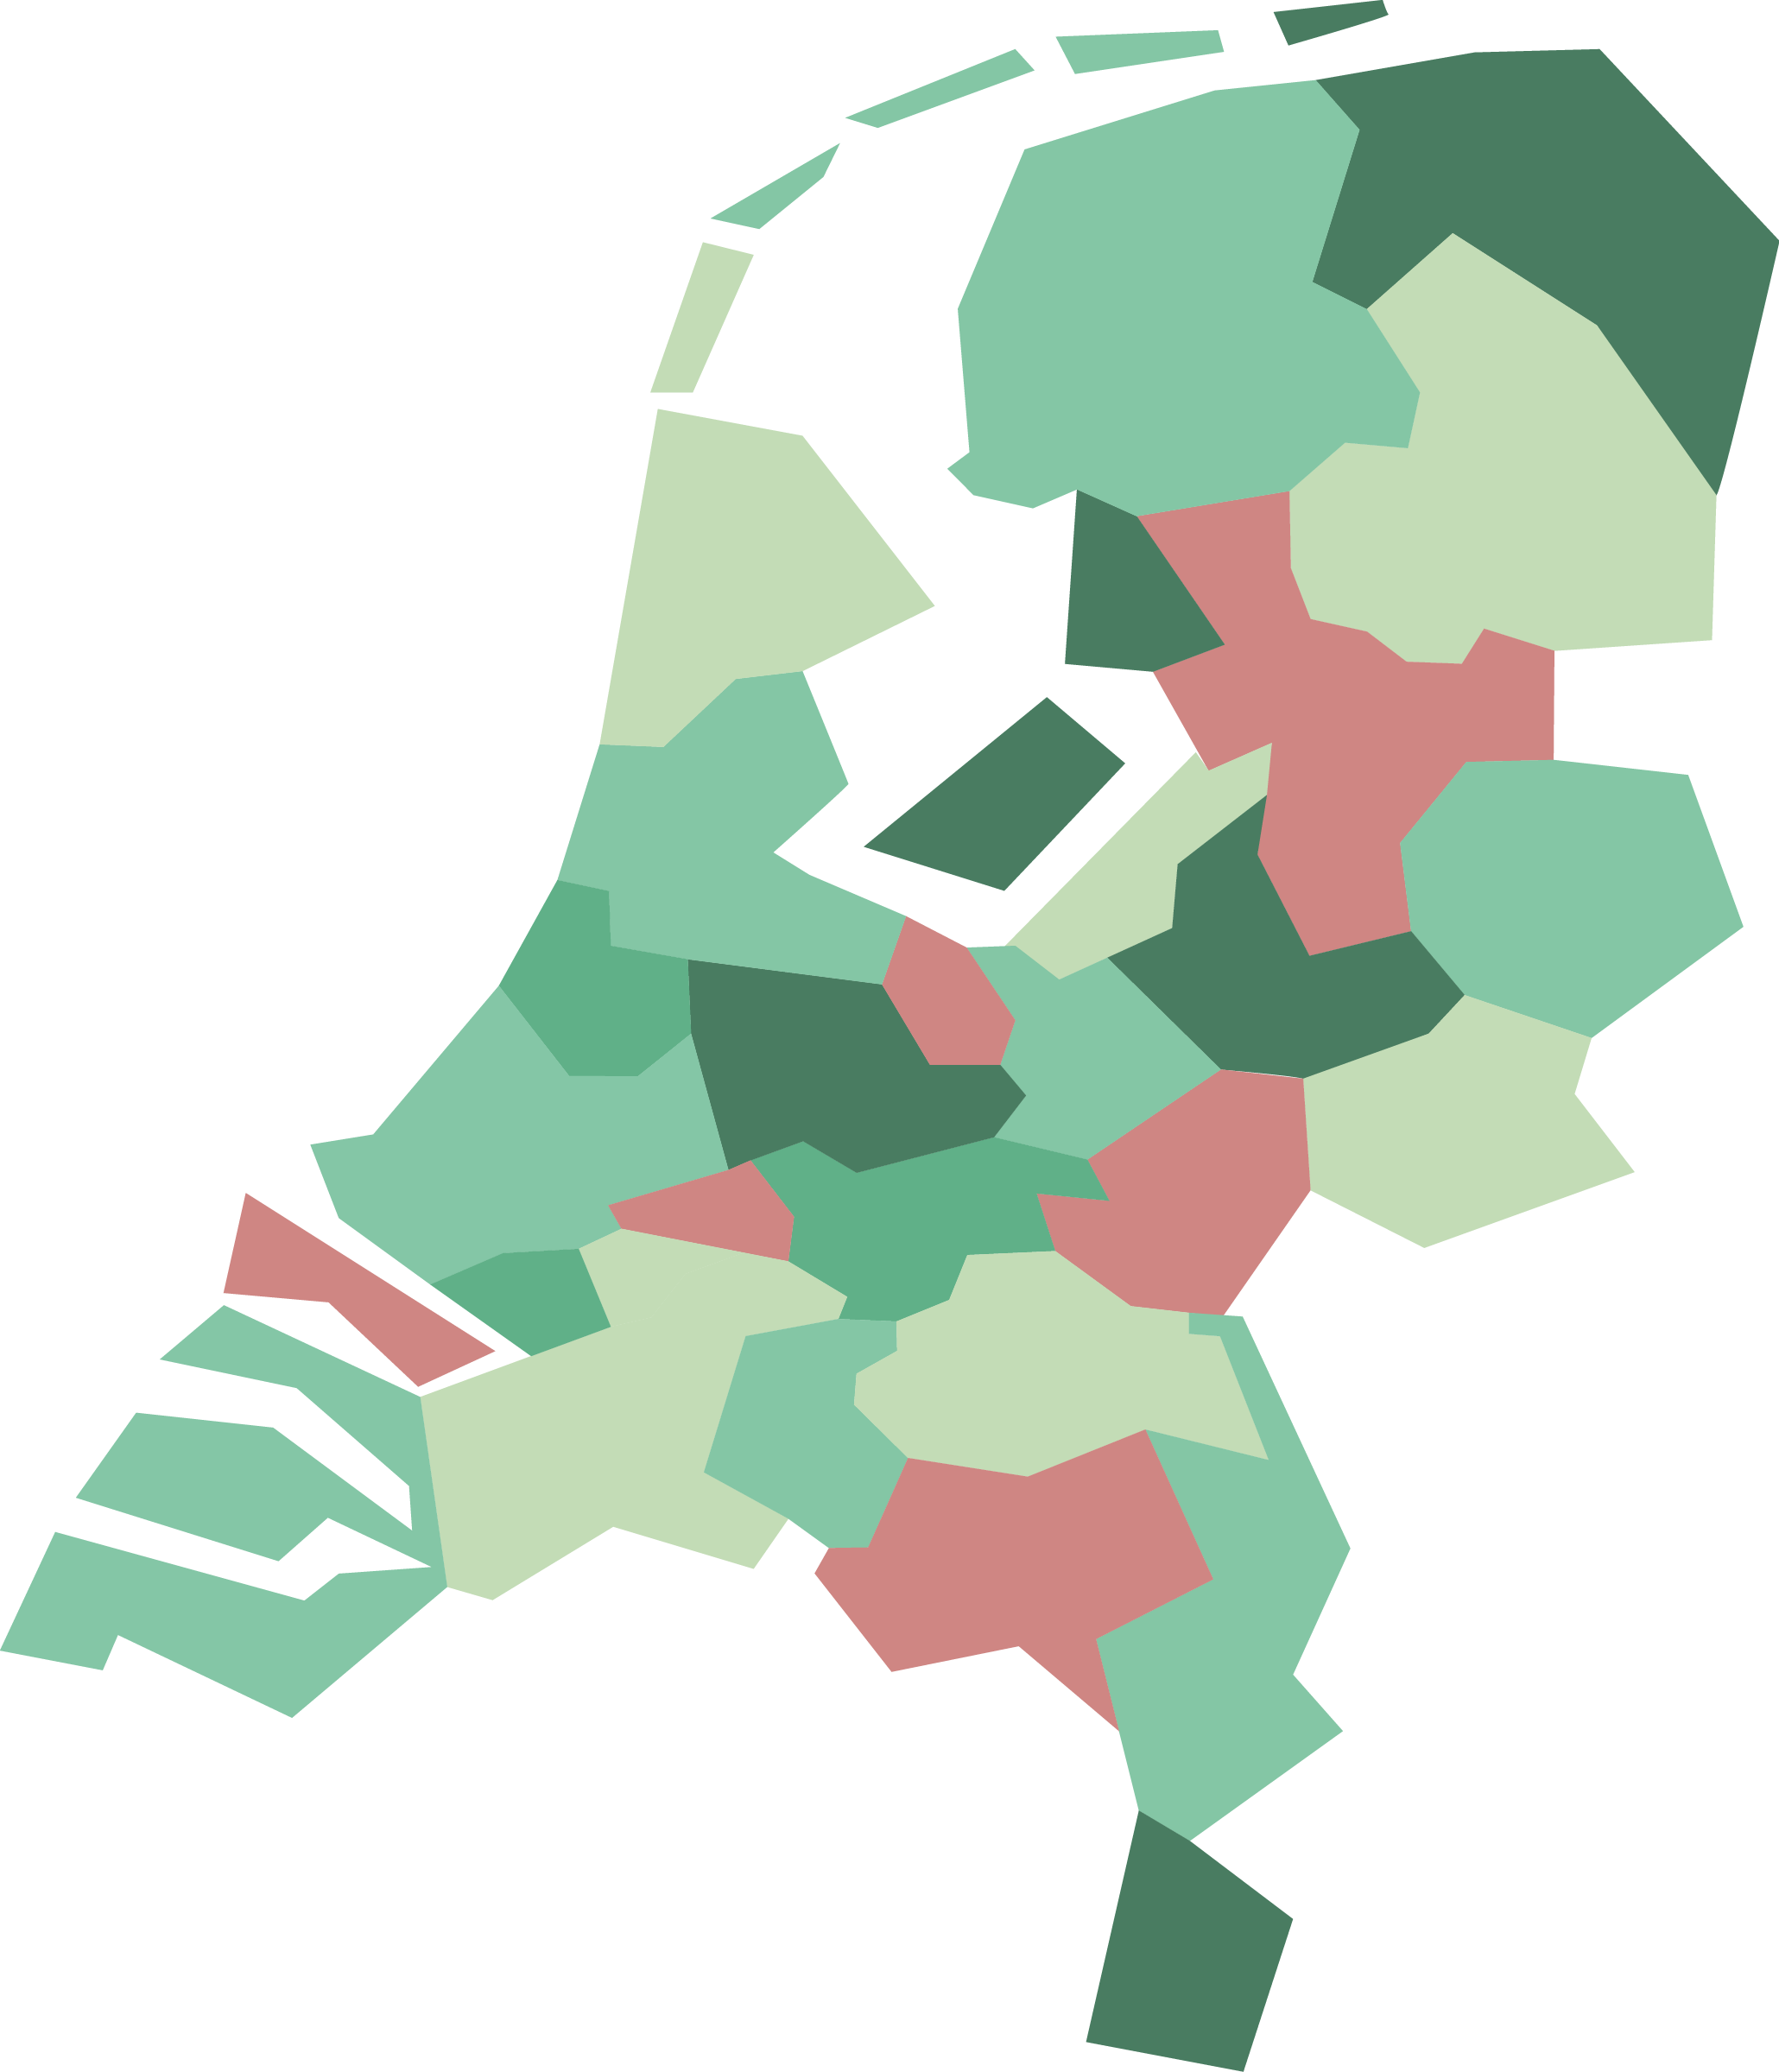
\includegraphics[width=.8\columnwidth]{img/energie/rol-van-de-res-kaart}
	\end{center}
	\textbf{\textit{Kaart met de 30 regio's \parencite{nationaal_programma_res_handreiking_2019}.}}
\end{figure}

\paragraph{De urgentie mist}
De gepresenteerde RES'en geven vooral invulling aan de in het klimaatakkoord gestelde doelen over de hoeveelheid duurzaam op te wekken elektriciteit.
Zowel in het klimaatakkoord als in de RES'en lijkt het hoofddoel van ambitieus klimaatbeleid echter buiten beeld te blijven: reageren op klimaatverandering en het bouwen van een toekomstbestendige wereld. Bij het opstellen van het klimaatakkoord was dan ook geen enkele wetenschappelijke expert betrokken \parencite{kropman_hoe_2019}.

Het gestelde doel voor elektriciteit was om in 2030 landelijk 35 terawattuur (TWh) stroom op te wekken met zonnedaken, zonneweides en windparken op het Nederlandse vasteland. Dat is circa 30 procent van het huidige landelijke stroomverbruik.
Door de verwachting dat het elektriciteitsverbruik de komende jaren zal stijgen, is de ambitie binnen de RES echter te laag.
Daarnaast lukken ook niet alle plannen altijd, door bijvoorbeeld technische beperkingen en tegenslag, juridische procedures, gebrek aan interesse bij ondernemers, problemen met vergunningen of door een tekort aan vakspecialisten.

Er zijn nu geen maatregelen of sancties als men niet aan de opgave voldoet.
Nederland doet het al het slechtst van alle landen in Europa wat betreft duurzame energie en is één van de grootste vervuilers per hoofd van de bevolking. Doordat er de afgelopen jaren nauwelijks tot concrete actie is overgegaan binnen de RES, maar vooral is overlegd, raakt Nederland nog verder achterop.

\paragraph{Gebrek aan overkoepelende visie}
In de RES’en wordt voorbijgegaan aan het complexe vraagstuk dat klimaatverandering voor een regio is. Er zijn afhankelijkheden tussen de regio’s, bijvoorbeeld in het gebruik van restwarmte van de industrie over regiogrenzen heen. Er zijn ook gerelateerde vraagstukken: de afname van biodiversiteit, toenemende woningnood, verduurzaming van de landbouw en voedselindustrie, Europese verplichtingen, en het stikstof-dossier. De gemeenten lijken de visie te missen om de RES als overkoepelend instrument te gebruiken om de klimaatcrisis tegen te gaan.

\paragraph{Draagvlak ontbreekt}
Het draagvlak voor de RES-beslissingen van provincies en gemeenten is minimaal, zeker bij de inwoners. Er was in het RES-proces weinig invloed van de volksvertegenwoordigers in de gemeenteraden \parencite{prins_eis_2020}. De inwoners, die dit moeten betalen en de gevolgen zullen merken, zijn tot nu toe nauwelijks betrokken. De RES’en zijn vooral ideeën van bestuurders, ambtenaren en ondernemers.

\paragraph{Hoe het anders kan}
Er zijn in Nederland gelukkig inspirerende voorbeelden hoe de besluitvorming anders kan.
Zo is in de gemeente Wijk bij Duurstede het beleid voor zonnevelden via een open proces opgesteld. Er ontstond een mooi voorbeeld van samenspel tussen inwoners en volksvertegenwoordigers. Een burgerpanel, samengesteld door loting met een evenredige verdeling over de drie kernen in het betreffende gebied, heeft de gemeenteraad geadviseerd over het te voeren energiebeleid. Dit advies is vervolgens door de raad overgenomen en vormt daarmee het kader waarbinnen voorstellen voor concrete projecten ingediend kunnen worden bij de gemeente \parencite{burgerpanel_zonnevelden_wijk_bij_duurstede_advies_2019}.
In Kampen vond een energietop plaats voor inwoners, bedrijven en raadsleden. En in de regio Drechsteden waren er waren regionale bijeenkomsten waar volksvertegenwoordigers, inwoners, bedrijven en stakeholders met elkaar in gesprek konden over energiescenario’s.

\todo{
\paragraph{Over de grens}
Franse burgerconventie

De Franse burgerconventie over het klimaat laat zien dat het mogelijk is om gedegen klimaatbeleid te ontwikkelen (NRC 2020-2). Het beraad maakt gebruik van democratie in de volle breedte en zorgt dat alle kennis, creativiteit en verantwoordelijkheidsgevoel in de samenleving wordt benut. Laten we het Franse voorbeeld (en dat van Wijk bij Duurstede) volgen. We doorbreken zo de impasse rond klimaatbeleid en maken onze democratie geschikt voor de eenentwintigste eeuw.

% \url{https://www.nrc.nl/nieuws/2020/07/03/laat-burgers-politici-helpen-organiseer-een-burgerberaad-a4004913#/handelsblad/2020/07/04/#204} (NRC 2020-2)

}

\paragraph{De waarde van burgerberaden}
Burgerberaden zijn een uitermate geschikt instrument om participatie en inspraak van burgers over het energiebeleid vorm te geven.
De beraden stellen over het algemeen adequate, haalbare en rechtvaardige maatregelen voor. De deelnemers vertegenwoordigen immers geen politieke partij en hoeven dus geen rekening te houden met verkiezingen, gunstige media-aandacht of een achterban. Partijpolitiek en lobbygroepen hebben weinig tot geen invloed op de besluitvorming van het burgerberaad, onder andere doordat de uitvoering in handen is van een onafhankelijke organisatie. En anders dan bij een referendum of enquête staat deliberatie centraal. Dat zorgt ervoor dat mensen voorbij ideologische, culturele en religieuze verschillen leren kijken en afgaan op feiten. De deelnemers krijgen tijd, informatie van experts en professionele gespreksbegeleiding, wat ze helpt in gesprek te gaan over complexe onderwerpen en tot constructieve, weldoordachte aanbevelingen te komen.
\todo{Hiermee geven we een invulling aan Remkes \parencite{staatscommissie_parlementair_stelsel_lage_2018}}

\todo{balans nationaal-regionaal. Hoe houden we nationaal overzicht en regionaal handelingsperspectief?}

\end{overwegingen}

\begin{aanbevelingen}
\speerpunt{We stellen een Nationaal Klimaatberaad in} om klimaatmaatregelen vast te stellen die ons beschermen tegen een onnodige verdere stijging van de temperatuur en de potentieel catastrofale gevolgen daarvan.

\speerpunt{We stellen regionale burgerberaden in} om voorstellen voor de regionale energietransitie op te stellen.

\end{aanbevelingen}

\end{multicols*}

\end{voorstel}


% extra
% \begin{voorstel}{De ideale energiemix}\end{voorstel}
% \begin{voorstel}{Verzwaren energienet}
\meeschrijver{Roelof Lanting}

\begin{samenvatting}
Tussen nu en 2030 zal er veel moeten veranderen in verband met het transport van elektriciteit, gas en waterstof (en mogelijk ook van andere energiedragers). Daarbij gaat het niet alleen om het energienet zelf (de techniek). Ook de besluitvorming over dat netwerk moet beter en - vanaf 2023 wellicht - anders. plaatsvinden.

Bij het energienet gaat om een zeer belangrijke voorwaarde om in 2030 energieneutraal te zijn. De bijdrage aan dat resultaat per 2030 en de politieke verantwoordelijkheid daarvoor zijn het onderwerp van dit voorstel.

Voor een CO2-neutrale energiesituatie in 2030 moet het nu bestaande elektriciteitsnet aangepast en ook uitgebouwd worden.

Als de netbeheerders er per eind 2022 niet toe bereid en in staat lijken om dat te doen, zullen er wijzigingen moeten komen in hun positie en in de regelingen waarop die positie berust.
\end{samenvatting}

\begin{uitdaging}
In 2021 en 2022 de beslissingen nemen die maken dat de ombouw van het elektriciteitsnet per 2030 gerealiseerd kan zijn..
\end{uitdaging}

\begin{overwegingen}
Het elektriciteitsnet heeft twee hoofdroutes, namelijk hoogspanning, ingericht door het Duits-Nederlandse staatsbedrijf Tennet en het net voor midden-/laagspanning. Daarvoor zijn drie netbeheerders verantwoordelijk : Enexsis, Liander en Stedin, elk in een aantal provincies. Deze bedrijven zijn monopolist en mogen geen andere bedrijvigheid ontplooien. Dit alles berust op de Elektriciteitswet. Naast leidingen zijn b.v ook verdeelstations onderdeel van die netten.

Het elektriciteitsnet (eigenlijk : de netten) is primair opgezet om in centrales (fossiel) opgewekte elektriciteit te transporteren.. Om daarnaast of in plaats daarvan ook decentraal uit wind en zon opgewekte elektriciteit blijkt het net nu al ontoereikend.

Voor de situatie in 2030 waarin volledig op zon “geleefd” wordt, zal het net dan ook aangepast moeten worden. Ook het omzetten van duurzaam opgewekte stroom in waterstof voor industrieel gebruik vereist aanpassingen.
Hoewel het al jaren duidelijk is dat deze aanpassingen nodig zijn, dralen de netbeheerders om die uit te voeren. Hun rol is de facto remmend.

In de CO2-neutrale situatie van 2030 wordt meer elektriciteit gebruikt dan nu, onder andere doordat het gasloos vervaardigen van goederen in veel situaties meer elektriciteit vergt.
Energiezuinigheid/besparen en de opwekking van stroom door inwoners/bedrijven zelf zullen die toename waarschijnlijk niet kunnen opvangen. Het net moet dus ook worden aangepast om meer elektriciteit van A naar B te brengen.

De sterke toename van het verbruik van stroom door datacentra compliceert de situatie ook nog eens (NOOT : zie NRC 22-6-2020, Dat verbruik overtreft dat van middelgrote steden. Hierover meer in Delta-voorstel … - titel - …. EINDE NOOT)

Dat de energieneutraliteit technisch grote veranderingen in de toestand, de capaciteit en de werking van het net nodig maken, staat vast.

Meer decentraal opwekken, gesloten systemen waterstof en andere (opslag-)technieken kunnen helpen, maar niet voldoende.

Welke veranderingen nodig zijn, is nog niet volledig duidelijk. Maar het zal sowieso veel kosten. . Netwerk- bedrijven noemen percentages (in 2030 wel 207 \% van de kosten in 2015) maar op basis van het huidige totale verbruik. En dat zal in 2030 groter zijn. Ze benadrukken hoe moeilijk het zal zijn en proberen geld op te halen, o.a. bij provincies.

Urgenda noemt in “Vijf keer anders” - niet onderbouwd - tot 2030 jaarlijks 2 \% van het BNP. Wat ook ontbreekt, is een onafhankelijke doorrekening. Die moet er in 2022 wel zijn.

Op het niveau van burgerinitiatieven is ondertussen al veel verduurzaming in gang gezet. . Industriële grootverbruikers voeren aanzienlijke veranderingen door moeten dat ook. Beide moeten zich kunnen baseren op heldere gegevens mbt een adekwaat net in 2030 en daarna.

Sinds 2004 (liberalisering, op aansturen van Europa) bouwen, beheren en exploiteren de net- beheerders het elektriciteitsnet, dus Tennet dat voor hoogspanning en Liander, Enexis en Stedin die voor midden- en laagspanning.

In de Elektriciteitswet komen mogelijkheden tot aansturing door de Minister van Economische Zaken voorkomen. Echter, de manier waarop de overheid tot nu toe haar bevoegdheden en positie in de praktijk gebruikt ten opzichte van de monopolistische bedrijven blijkt onvoldoende om de “omslag naar neutraal” te laten plaatsvinden. Mogelijk moeten die bevoegdheden ook worden uitgebreid. Maar omdat wijzigingen in organisatiestructuren en in wetgeving vertragend werken, kiezen we daar nu nog niet voor. Ze moeten alleen dan plaatsvinden als dat eind 2021 nodig en/of onvermijdelijk is gebleken. 

De liberalisering heeft teveel ruimte gecreëerd om niet te doen wat klaarblijkelijk nodig is. Daarom zal de overheid al meteen in 2021 een grotere rol moeten nemen en gebruik maken van bestaande bevoegdheden gebruiken.
\end{overwegingen}

\begin{aanbevelingen}
In de jaren 2021 en 2022 worden de mogelijkheden in de Elektriciteitswet  maximaal gebruikt om concreet te maken wat er technisch moet veranderen om in 2030 een elektriciteitsnet te krijgen dat duurzaam opgewekte elektriciteit kan transporteren naar waar het gebruikt wordt.

In 2022 wordt door het PBL een doorrekening  van de kosten van aanpassing van het net/de netten uitgevoerd, waarbij koppeling van gebruik voor waterstof en gas en andere opties meegenomen worden.

In de 2023 en de eerstvolgende jaren moeten de noodzakelijke veranderingen in het net (de netten) uitgevoerd worden. Het zal van de per eind  2021 gebleken handelingsbereidheid van de netbeheerders afhangen of zij in de laatste acht jaar tot 2031 in dezelfde positie als nu kunnen blijven.. Als dat niet het geval is , zal er in 2022 wijziging van de wetgeving moeten plaatsvinden.
\end{aanbevelingen}

\paragraph{Literatuur}
www.hoogspanningsnet

Vijf keer anders, uitgave van Urgenda

NRC 10-10-2019 (p. E6/7) en 14 mei 2020 (p. E 3)

\end{voorstel}

% \begin{voorstel}{Geothermie}
\meeschrijver{Rints Swart}

\begin{samenvatting}
Samenvatting
\end{samenvatting}

\begin{uitdaging}
Op diverse plekken in Nederland wordt aardwarmte met succes gebruikt voor de verwarming van kassen. De eerste aardwarmtewinning is in 2007 in Bleiswijk gerealiseerd. Verwarming van een kas met water van 60 graden Celsius afkomstig van 1700 meter diepte. .(Bron: Bosatlas van de Energie)

In Zwolle wordt in het kader van de energietransitie onderzoek gedaan naar de toepassing van geothermie voor de verwarming van reeds bestaande stadswijken, Holtenbroek en Aalanden.

Op deze schaalgrootte is dat in Nederland nog niet eerder onderzocht en toegepast.

In Frankrijk wordt al tientallen jaren zonder problemen warmte uit de aarde gebruikt voor woonwijken in de regio van  Parijs (zie: Geothermie en Ile-de-France en Geothermie a Villages Nature Paris).

De rijksoverheid (Planbureau voor de Leefomgeving) geeft op basis van de uitkomsten van het SCAN-onderzoek aan waar in Nederland geschikte locaties zijn om, gebruik makend van geothermische warmte, stadswijken te voorzien van warmte. (Zo ook bijvoorbeeld voor de stad Groningen). In 2022 zou een eerste landelijk beeld gegeven kunnen worden (Regie bij het Rijk).
\end{uitdaging}

\begin{overwegingen}
\paragraph{Uitleg aardwarmte}
Wat is aardwarmte en welke typen warmte onderscheiden we: geothermie, diepe geothermie en ultra diepe geothermie. 

Hoe dieper we de warmte oppompen hoe warmer het water is.

Voor verwarming van woningen en kantoren is een warmte van 45 graden Celsius voldoende.

Voor de glastuinbouw wordt 70 graden op prijs gesteld. 
Voor de industrie …

Water van meer dan 100 graden kan een elektrische centrale bedienen.

Daarnaast is uitleg van WKO-systemen (warmte-koude opslag) verstandig (www.wkotool.nl).

Er is al veel bekend over de ondergrond van Nederland met watervoerende aardlagen ( zie kaarten van 2 km diepte en 5 km diepte.

Momenteel vindt seismisch onderzoek plaats om ontbrekende gedeelten van de ondergrond nauwkeuriger in beeld te krijgen: SCAN = Seismische Campagne Aardwarmte Nederland.

In de glastuinbouw worden goede resultaten behaald: Bleiswijk, Koekoekspolder (IJsselmuiden).

In Zwolle wordt in het kader van de Regionale Energie Strategie (RES) een pilot-project uitgevoerd voor de verwarming van bestaande woonwijken. Een proefboring zal volgend jaar plaatsvinden.

In eerste instantie zijn proefboringen een dure aangelegenheid omdat roestvrijstalen buizen nodig zijn. Er zijn per locatie twee buizen nodig om het warme water op te pompen en daarna via een andere buis terug te pompen.

In tegenstelling tot de winning van schaliegas vindt nauwelijks verontreiniging van de ondergrond plaats. Bij de winning van schaliegas is het grote probleem dat het verontreinigde water eerst in basins weer schoongemaakt moet worden. Bovendien wordt daarbij met explosies de gasvoerende lagen gebroken. Bij aardwarmte gaat het om goed watervoerende lagen die afgedekt zijn door ondoorlatende kleilagen. In de buizen worden kleine pompen aangebracht die op zich energie behoeven, elektriciteit). Bij de projecten voor de glastuinbouw is gebleken dat de daarvoor benodigde energie ruimschoots de besparende elektriciteit door de warmtewisselaar overtreft. In het opgepompte water wordt wel zout gewonnen.

De warmtenetten bij de glastuinbouw zijn van korte lengte, wat bij grote woningbouwprojecten niet het geval is. Bij glastuinbouw is het een gezamenlijk initiatief van ondernemende tuinders..Voor de proefboringen is het de overheid die dat grotendeels financiert. Bij de Koekoekspolder is dat de provincie Overijssel. Na enkele problemen is er nu zelfs sprake van uitbreiding van het aantal hectare kassen. In het geval van een complete woonwijk is het de gemeente die aanvankelijk de regie voert. Daarbij wordt ze bijgestaan door deskundigen van EBN, TNO en adviesbureaus.

Bij de glastuinbouw is gebleken dat de kosten van boringen en continue energie voor pompen e.d. op termijn terugverdiend kunnen worden.

Geothermie in de glastuinbouw stimuleren.
Voor de verwarming van stadswijken verder onderzoek doen en toepassen.

\paragraph{Uitleg}
De hete kern van de aarde is een vrijwel onuitputtelijke bron van aardwarmte. Op 2 kilometer diepte heeft grondwater in Nederland gemiddeld al een temperatuur van meer dan 70 graden Celsius. Met opgepompt grondwater van meer dan 45 graden C kun je huizen en kassen verwarmen, boven de 120 graden Celsius kun je mogelijk elektriciteit opwekken. De potentie voor de winning van aardwarmte is o.a. afhankelijk van de temperatuur van het grondwater, de dikte en doorlatendheid van de watervoerende laag.

\paragraph{Geothermie in de tuinbouw}
Voor verwarming van tuinbouwkassen zijn reeds diverse voorbeelden te noemen, waaronder in de Koekoekspolder bij IJsselmuiden.

\paragraph{Verwarming woonwijken}
Het project in Zwolle is een van de eerste grootschalige toepassingen van geothermie voor de verwarming van bestaande woonwijken. Het is een pilot-project en de ervaringen die ermee worden opgedaan kunnen elders in Nederland van nut zijn. Het succes hangt af van de ligging van warm water in de aardlagen onder de plek waar de warmte gebruikt wordt.

Geologisch onderzoek van de bodem in Nederland heeft reeds een beeld opgeleverd dat toepassing van aardwarmte mogelijk maakt. Zie kaarten:

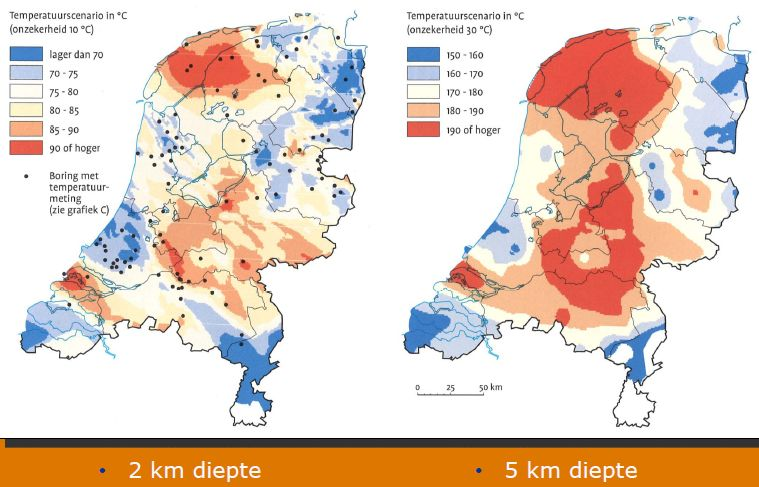
\includegraphics[width=.5\textwidth]{img/energie/geothermie-temperatuurscenarios}
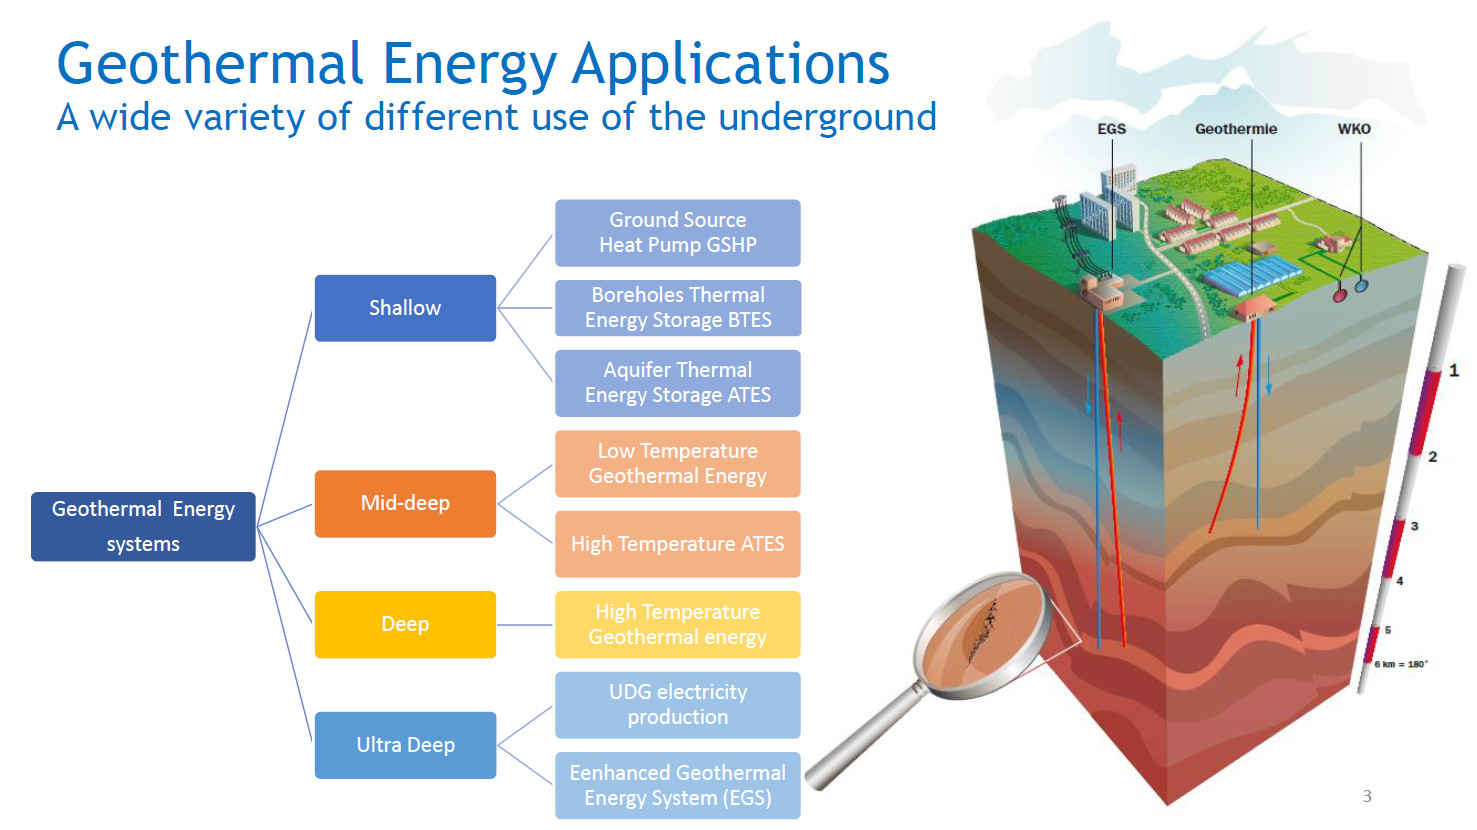
\includegraphics[width=.5\textwidth]{img/energie/geothermie-applications}

\paragraph{Aardwarmte}
De kern van de aarde bevat een onuitputtelijke hoeveelheid warmte. Op 2  kilometer diepte heeft grondwater in Nederland al een temperatuur van meer dan 70 graden Celsius.

Aardwarmte of geothermie (Grieks geo, aarde en thermos, warmte) is thermische energie, warmte, uit de Aarde.

Geothermie is een duurzame warmtebron en een van de mogelijkheden om aardgas te vervangen. Een geothermiebron kan jaarlijks de warmte produceren voor circa 10.000 woningen, ongeveer 02,20 PJ/jaar (Bron: www.geothermie.nl) afhankelijk van de geologische situatie ter plekke van de boringen.

\paragraph{Pilot-project Zwolle}
Zwolle Noord blijkt redelijk kansrijk voor de realisatie van een geothermiebron. Woningcorporaties hebben de intentie uitgesproken om die warmte af te nemen.

In het kader van het Europees subsidieprogramma “Geothermica” heeft Nederland via TNO een aanvraag gedaan voor een onderzoeksproject “Result”. Dit subsidieprogramma is gericht op onderzoek naar het toepassen van slimme boortechnieken in zogenaamde marginale reservoirs geothermie. De voor-aanvraag is onlangs door de Geothermica-organisatie van de EU gehonoreerd. In 2021 zal de eerste boring plaatsvinden in de Dijkslanden in Zwolle. Na een succesvolle boring bij deze productieput zal een tweede boring uitgevoerd worden, de injectieput. In 2023 zou dan de eerste winning plaats kunnen vinden.

Een proefboring geeft zekerheid over de geologische omstandigheden en helpt om het bronvermogen van de locatie te bepalen. De zekerheid van het vermogen is van groot belang om de investeringsbereidheid in de ontwikkeling van een warmtenet.

\paragraph{VERKLARINGEN, INSTANTIES, ADVIESBUREAUS}
SCAN    Seismische Campagne Aardwarmte Nederland

DAGO    Dutch Association Geothermal Operators

EBN    Energie Beheer Nederland

SodM    Staatstoezicht op de Mijnen

TNO    Nederlands Instituut voor Toegepast Natuurwetenschappelijk Onderzoek

Firan    Ontwerpt, realiseert, financiert en beheert toekomstbestendige energie-infrastructuur

IF Technology    Adviesbureau Geothermie, Bodemenergie , Aquathermie

Geotherm Energy Systems    Pionier op het gebied van bodemenergie en WKO

CE Delft        Onderzoeks- en adviesbureau op het gebied van milieu- en duurzaamheidsvraagstukken

Kas als Energiebron    Streeft ernaar het aantal gerealiseerde projecten per jaar te vergroten

Stichting Warmtenetwerk

Platform Geothermie

Masterplan Aardwarmte
\end{overwegingen}

\begin{aanbevelingen}
Toepassing van aardwarmte In de glastuinbouw is succesvol gebleken. In combinatie met ondergrondse opslag van CO2 en Warmte-Koude Opslag in de omgeving van glastuinbouwgebieden, zoals het Westland, betekent dat een enorme energiebesparing in vergelijking met confessionele methoden.

Het project in Zwolle betreffende toepassing van geothermie voor de verwarming van woonwijken zal kennis en ervaring opleveren voor bredere toepassing in Nederland.  Het SCAN-onderzoek dat momenteel gaande is zal uit  kunnen wijzen waar geothermie verder geschikt is voor bestaande en nieuwe woonwijken. De ontwikkelingen nauwgezet in de gaten houden. Aan de huidige boortechnieken en recente kennis en onderzoek zal het niet liggen hoe snel een en ander bredere toepassing vindt. Het SCAN-onderzoek loopt nog. Het is veeleer een organisatie-vraagstuk en het nemen van verantwoordelijkheden. Er is een fase van onderzoek en het verrichten van boringen met de nodige financiele risico’s en daarna aanleg, beheer en onderhoud van het leidingen-netwerk. 

Woningcorporaties willen wel meedoen, maar willen dan wel de zekerheid hebben dat er garanties zijn voor warmtelevering, anders kiezen ze voor warmtepompen en koude-warmte opslag per woning of woningblok. In het laatste geval behouden ze zelf de regie.
\end{aanbevelingen}

\paragraph{Literatuur}
Zwolle geeft energie, plan van aanpak 2018-2022

Voortgang geothermie, informatienota voor de raad, van Zwolle, januari 2020

De Bosatlas van de Energie, Noordhoff  Uitgevers Groningen

De Bosatlas van de Duurzaamheid, Noordhoff Uitgevers, Groningen

https://www.geothermie.nl

https://www.rijksoverheid.nl/onderwerpen/duurzame-energie/aardwarmte

https://www..iftechnology.nl/geothermie

https://vito.be/nl/diepe-geothermie

https://www.kasalsenergiebron.nl/duurzame-energie/aardwarmte

Wikipedia: Geothermie en Ile-de-France

La Geothermie a Villages Nature Paris (videofilms)

De Geo, Aarde, Klimaatvraagstukken, Studieboek VWO, ThiemeMeulenhoff, Amersfoort
\end{voorstel}

% \begin{voorstel}{Opslag}\end{voorstel}
% \begin{voorstel}{\COO-belasting}\end{voorstel}

\thema{Vervoer}

\begin{voorstel}{Visie op vervoer}\end{voorstel}

\begin{voorstel}{Terugdringen van verplaatsingen}\end{voorstel}
\begin{voorstel}{Auto’s}\end{voorstel}
\begin{voorstel}{Busjes en vrachtwagens}\end{voorstel}
\begin{voorstel}{Rekeningrijden}\end{voorstel}
\begin{voorstel}{Vliegverkeer}\end{voorstel}
\begin{voorstel}{Scheepvaart}\end{voorstel}
\begin{voorstel}{Openbaar vervoer}\end{voorstel}
\begin{voorstel}{Europees treinnetwerk}\end{voorstel}
\thema{Gebouwen}

\voorstel{Visie op gebouwde omgeving}

\voorstel{Van het gas af}
\voorstel{Huizen isoleren}
\voorstel{Energiezuinige huishoudens}
\voorstel{Energieneutrale/zelfvoorzienende huizen}
\voorstel{Gebouwen}
\voorstel{Warmtenet}
\voorstel{Aquathermie}
\voorstel{Iedereen investeert (verplicht maar goedkoop)}
\voorstel{Rol van wooncorporaties}
\voorstel{Bouw van honderdduizenden klimaatneutrale woningen}
 
\thema{Land \& Natuur}

\begin{visie-concept}{Visie op land en natuur}\end{visie-concept}

\begin{voorstel-concept}{Verminderen dierlijke consumptie}\end{voorstel-concept}
\begin{voorstel-concept}{Voedselverspilling tegengaan}\end{voorstel-concept}
\begin{voorstel-concept}{Duurzame veeteelt}\end{voorstel-concept}
\begin{voorstel-concept}{Duurzame landbouw}\end{voorstel-concept}
\begin{voorstel-concept}{Duurzame tuinbouw}\end{voorstel-concept}
\begin{voorstel-concept}{Biodiversiteit}\end{voorstel-concept}
\begin{voorstel-concept}{Natuur}\end{voorstel-concept}
\begin{voorstel-concept}{(Her)bebossing}\end{voorstel-concept}
\begin{voorstel-concept}{Veenlanden als koolstofopslag}\end{voorstel-concept}
\begin{voorstel-concept}{Groen in de stad}\end{voorstel-concept}
\begin{voorstel-concept}{Frisse lucht, schone grond, helder water}\end{voorstel-concept}
\thema{Industrie \& Grondstoffen}

\begin{visie-concept}{Visie op industrie en grondstoffen}\end{visie-concept}

\begin{voorstel-concept}{Terugdringen consumptie}\end{voorstel-concept}
\begin{voorstel-concept}{Haven}\end{voorstel-concept}
\begin{voorstel-concept}{Staal}\end{voorstel-concept}
\begin{voorstel-concept}{Petrochemie}\end{voorstel-concept}
\begin{voorstel-concept}{Kunststoffen}\end{voorstel-concept}
\begin{voorstel-concept}{Kunstmest}\end{voorstel-concept}
\begin{voorstel-concept}{Overige chemie}\end{voorstel-concept}
\begin{voorstel-concept}{Hout- en bouwmaterialen}\end{voorstel-concept}
\begin{voorstel-concept}{Alternatieve materialen}\end{voorstel-concept}
\begin{voorstel-concept}{Hergebruik restwarmte}\end{voorstel-concept}
\begin{voorstel-concept}{Koolstofafvang en -hergebruik (CCS \& CCU)}\end{voorstel-concept}
\begin{voorstel-concept}{Vuilstortplaatsen}\end{voorstel-concept}
\begin{voorstel-concept}{Circulaire economie}\end{voorstel-concept}
\begin{voorstel-concept}{Reparatie}\end{voorstel-concept}

\thema{Arbeid \& Scholing}

\begin{visie-concept}{Visie op arbeid en scholing}\end{visie-concept}

\begin{voorstel-concept}{De ideale arbeidsmarkt}\end{voorstel-concept}
\begin{voorstel-concept}{Het capaciteitsorgaan}\end{voorstel-concept}
\begin{voorstel-concept}{Groene omscholing}\end{voorstel-concept}
\begin{voorstel-concept}{Meer vrouwen in technische beroepen}\end{voorstel-concept}
\begin{voorstel-concept}{30-urige werkweek}\end{voorstel-concept}
\begin{voorstel-concept}{Groene baangarantie}\end{voorstel-concept}
\begin{voorstel-concept}{Groen basisinkomen}\end{voorstel-concept}
\begin{voorstel-concept}{Groene arbeidsmigratie}\end{voorstel-concept}
\begin{voorstel-concept}{Klimaatcurriculum}\end{voorstel-concept}

\thema{Geld \& Economie}

\voorstel{Visie op geld en economie}

\voorstel{Belastinghervorming}
\voorstel{Uitstootheffing}
\voorstel{Geen fossiele investeringen}
\voorstel{Tegengaan belastingontwijking}
\voorstel{De centrale bank als groene geldschepper}
\voorstel{Publieke bank}
\voorstel{Reclamevrije wereld}

\thema{Technologie \& Innovatie}

\begin{visie-concept}{Visie op technologie en innovatie}\end{visie-concept}

\begin{voorstel-concept}{Industriepolitiek}\end{voorstel-concept}
\begin{voorstel-concept}{Een nieuwe onderzoeksagenda}\end{voorstel-concept}
\begin{voorstel-concept}{Groen investeringsfonds}\end{voorstel-concept}
\begin{voorstel-concept}{Expeditie waterstof}\end{voorstel-concept}
\begin{voorstel-concept}{Visie voor een nieuw Bell Labs}\end{voorstel-concept}
\begin{voorstel-concept}{Toekomstgeluid}\end{voorstel-concept}

\thema{Democratie \& Bestuur}

\begin{visie-concept}{Visie op democratie en bestuur}\end{visie-concept}

\begin{voorstel-concept}{Minister van Klimaat en Energie}\end{voorstel-concept}
\begin{voorstel-concept}{De Klimaatraad}\end{voorstel-concept}
\begin{voorstel-concept}{Rol van de Regionale Energiestrategie}\end{voorstel-concept}
\begin{voorstel-concept}{Burgerinspraak}\end{voorstel-concept}
\begin{voorstel-concept}{Stimuleren lokale energiecoöperaties}\end{voorstel-concept}
\begin{voorstel-concept}{Vrijheid voor lokale initiatieven}\end{voorstel-concept}

\themaconcept{Klimaatadaptatie}

\begin{visie-concept}{Visie op klimaatadaptatie}\end{visie-concept}

\begin{voorstel-concept}{Kustbescherming}\end{voorstel-concept}
\begin{voorstel-concept}{Rivieren}\end{voorstel-concept}
\begin{voorstel-concept}{Droogte voorkomen en oplossen}\end{voorstel-concept}
\begin{voorstel-concept}{Verzilting}\end{voorstel-concept}
\begin{voorstel-concept}{Bodemdaling}\end{voorstel-concept}
\begin{voorstel-concept}{Regenbestendige steden}\end{voorstel-concept}
\begin{voorstel-concept}{Koele steden}\end{voorstel-concept}

\thema{Internationale Ontwikkelingssamenwerking}

\begin{voorstel}{Visie op internationale ontwikkelingssamenwerking}\end{voorstel}

\begin{voorstel}{Ondersteunen internationale klimaatadaptatie}\end{voorstel}
\begin{voorstel}{Eerlijke bijdrage Green Climate Fund}\end{voorstel}
\begin{voorstel}{Compensatie voor gevolgen klimaatverandering}\end{voorstel}
\begin{voorstel}{Ecocide strafbaar stellen}\end{voorstel}
\begin{voorstel}{Garanderen van eerlijke materialen}\end{voorstel}
\begin{voorstel}{Duurzame certificering}\end{voorstel}
\begin{voorstel}{Stimuleren duurzame landbouw}\end{voorstel}
\begin{voorstel}{Onderwijs voor meisjes}\end{voorstel}
\begin{voorstel}{Vrouwen betrekken bij vergroening}\end{voorstel}



% \printbibliography
\end{document}
